\documentclass[12pt,addpoints]{exam}
\usepackage{amsmath, amssymb, amsthm, enumerate, graphicx}
\usepackage[usenames,dvipsnames]{color}
\usepackage{todonotes}
\usepackage{bm}
\usepackage[colorlinks=true,urlcolor=blue]{hyperref}
\usepackage{geometry}
\geometry{margin=1in}
\usepackage{float}
\usepackage{graphics}
\setlength{\marginparwidth}{2.15cm}
\usepackage{booktabs}
\usepackage{enumitem}
\usepackage{epsfig}
\usepackage{setspace}
\usepackage{parskip}
\usepackage[normalem]{ulem}
\usepackage{tikz}
\usetikzlibrary{positioning, arrows, automata}
\usepackage{pgfplots}
\usepgfplotslibrary{fillbetween}
\usepackage[font=scriptsize]{subcaption}
\usepackage{float}
\usepackage{algorithmicx}
\usepackage[noend]{algpseudocode}
\usepackage{environ}
\usepackage{bbm}
\usepackage{graphicx}
\usepackage{titling}
\usepackage{url}
\usepackage{xcolor}
\usepackage{lipsum}
\usepackage{lastpage}
\usepackage[colorlinks=true,urlcolor=blue]{hyperref}
\usepackage{multicol}
\usepackage{tabularx}
\usepackage{comment}
\usepackage{amsmath}
\usepackage{nicefrac}
\usepackage[tableposition=top]{caption}
\usepackage[many]{tcolorbox}
\usepackage{colortbl}
\usepackage{array}
\usepackage{multirow}
\usepackage{listings}
\usepackage{color}
\usepackage{adjustbox}
\usepackage{wasysym} % For \CIRCLE
\usepackage{cancel} % For \xcancel

\pgfplotsset{compat=1.16}


\definecolor{dkgreen}{rgb}{0,0.6,0}
\definecolor{gray}{rgb}{0.5,0.5,0.5}
\definecolor{mauve}{rgb}{0.58,0,0.82}

\lstset{frame=tb,
  language=Python,
  aboveskip=3mm,
  belowskip=3mm,
  showstringspaces=false,
  columns=flexible,
  basicstyle={\small\ttfamily},
  numbers=none,
  numberstyle=\tiny\color{gray},
  keywordstyle=\color{blue},
  commentstyle=\color{dkgreen},
  stringstyle=\color{mauve},
  breaklines=true,
  breakatwhitespace=true,
  tabsize=3
}


\newcommand{\class}{10-301/601 Machine Learning}
\newcommand{\term}{Spring 2023}
\newcommand{\examnum}{Exam 2}
\newcommand{\examdate}{11/09/2023}
\newcommand{\timelimit}{120 minutes}
\newcommand{\argmax}{\operatornamewithlimits{arg\,max}}
\newcommand{\argmin}{\operatornamewithlimits{arg\,min}}

% Instead of lines, use blank space.
%\renewcommand{\fillwithlines}[1]{\vspace{#1}}

\def\x{\mathbf x}
\def\y{\mathbf y}
\def\w{\mathbf w}
\def\v{\mathbf v}
\def\E{\mathbb E}
\def\V{\mathbb V}
\def\a{\mathbf a}
\def\z{\mathbf z}

\newcommand\MyBox[1]{%
  \fbox{\parbox[c][1.7cm][c]{1.7cm}{\centering #1}}%
}
\newcommand\MyVBox[1]{%
  \parbox[c][1.7cm][c]{2.5cm}{\centering\bfseries #1}%
}  
\newcommand\MyHBox[2][\dimexpr1.7cm+2\fboxsep\relax]{%
  \parbox[c][1cm][c]{#1}{\centering\bfseries #2}%
}  
\newcommand\MyTBox[3]{
  \MyVBox{#1}\MyBox{#2}
  \MyBox{#3}\par
}


\newcommand{\pts}[1]{(#1 points)}

% SOLUTION environment
\newenvironment{soln}{\leavevmode\color{red}\ignorespaces }{}

% QUESTION AUTHORS environment
\newenvironment{qauthor}{\leavevmode\color{blue}\ignorespaces }{}

% Question tester comment environment
\newenvironment{qtester}{\leavevmode\color{green}\ignorespaces}{}

% TO ONLY SHOW HOMEWORK QUESTIONS, include following (else comment out):
   % \RenewEnviron{soln}{}
   \RenewEnviron{qauthor}{}
  \RenewEnviron{qtester}{}

\newcommand{\norm}[1]{\lVert #1 \rVert}
\newcommand{\st}{\mathrm{s.t.}}

\makeatletter
\newcommand{\removelatexerror}{\let\@latex@error\@gobble}
\makeatother

\setlength\linefillheight{.35in}

%%%%%%%%%%%%%%%%%%%%%%%%%%%%%%%%%%%%%%%%%%
% Custom commands                        %
%%%%%%%%%%%%%%%%%%%%%%%%%%%%%%%%%%%%%%%%%%

% First argument is width, second argument is label.
\newcommand{\blankforFITB}[2]{\underline{\hspace{#1}#2\hspace{#1}}}

\newcommand{\vc}[1]{\boldsymbol{#1}}

\newcommand{\fpartial}[2]{\frac{\partial #1}{\partial #2}}
\newcommand{\adj}[1]{\frac{\partial J}{\partial #1}}
\newcommand{\chain}[2]{\adj{#2} = \adj{#1}\frac{\partial #1}{\partial #2}}

% mathcal
\newcommand{\Ac}{\mathcal{A}}
\newcommand{\Bc}{\mathcal{B}}
\newcommand{\Cc}{\mathcal{C}}
\newcommand{\Dc}{\mathcal{D}}
\newcommand{\Ec}{\mathcal{E}}
\newcommand{\Fc}{\mathcal{F}}
\newcommand{\Gc}{\mathcal{G}}
\newcommand{\Hc}{\mathcal{H}}
\newcommand{\Ic}{\mathcal{I}}
\newcommand{\Jc}{\mathcal{J}}
\newcommand{\Kc}{\mathcal{K}}
\newcommand{\Lc}{\mathcal{L}}
\newcommand{\Mc}{\mathcal{M}}
\newcommand{\Nc}{\mathcal{N}}
\newcommand{\Oc}{\mathcal{O}}
\newcommand{\Pc}{\mathcal{P}}
\newcommand{\Qc}{\mathcal{Q}}
\newcommand{\Rc}{\mathcal{R}}
\newcommand{\Sc}{\mathcal{S}}
\newcommand{\Tc}{\mathcal{T}}
\newcommand{\Uc}{\mathcal{U}}
\newcommand{\Vc}{\mathcal{V}}
\newcommand{\Wc}{\mathcal{W}}
\newcommand{\Xc}{\mathcal{X}}
\newcommand{\Yc}{\mathcal{Y}}
\newcommand{\Zc}{\mathcal{Z}}

% mathbb
\newcommand{\Ab}{\mathbb{A}}
\newcommand{\Bb}{\mathbb{B}}
\newcommand{\Cb}{\mathbb{C}}
\newcommand{\Db}{\mathbb{D}}
\newcommand{\Eb}{\mathbb{E}}
\newcommand{\Fb}{\mathbb{F}}
\newcommand{\Gb}{\mathbb{G}}
\newcommand{\Hb}{\mathbb{H}}
\newcommand{\Ib}{\mathbb{I}}
\newcommand{\Jb}{\mathbb{J}}
\newcommand{\Kb}{\mathbb{K}}
\newcommand{\Lb}{\mathbb{L}}
\newcommand{\Mb}{\mathbb{M}}
\newcommand{\Nb}{\mathbb{N}}
\newcommand{\Ob}{\mathbb{O}}
\newcommand{\Pb}{\mathbb{P}}
\newcommand{\Qb}{\mathbb{Q}}
\newcommand{\Rb}{\mathbb{R}}
\newcommand{\Sb}{\mathbb{S}}
\newcommand{\Tb}{\mathbb{T}}
\newcommand{\Ub}{\mathbb{U}}
\newcommand{\Vb}{\mathbb{V}}
\newcommand{\Wb}{\mathbb{W}}
\newcommand{\Xb}{\mathbb{X}}
\newcommand{\Yb}{\mathbb{Y}}
\newcommand{\Zb}{\mathbb{Z}}

% mathbf lowercase
\newcommand{\av}{\mathbf{a}}
\newcommand{\bv}{\mathbf{b}}
\newcommand{\cv}{\mathbf{c}}
\newcommand{\dv}{\mathbf{d}}
\newcommand{\ev}{\mathbf{e}}
\newcommand{\fv}{\mathbf{f}}
\newcommand{\gv}{\mathbf{g}}
\newcommand{\hv}{\mathbf{h}}
\newcommand{\iv}{\mathbf{i}}
\newcommand{\jv}{\mathbf{j}}
\newcommand{\kv}{\mathbf{k}}
\newcommand{\lv}{\mathbf{l}}
\newcommand{\mv}{\mathbf{m}}
\newcommand{\nv}{\mathbf{n}}
\newcommand{\ov}{\mathbf{o}}
\newcommand{\pv}{\mathbf{p}}
\newcommand{\qv}{\mathbf{q}}
\newcommand{\rv}{\mathbf{r}}
\newcommand{\sv}{\mathbf{s}}
\newcommand{\tv}{\mathbf{t}}
\newcommand{\uv}{\mathbf{u}}
\newcommand{\vv}{\mathbf{v}}
\newcommand{\wv}{\mathbf{w}}
\newcommand{\xv}{\mathbf{x}}
\newcommand{\yv}{\mathbf{y}}
\newcommand{\zv}{\mathbf{z}}

% mathbf uppercase
\newcommand{\Av}{\mathbf{A}}
\newcommand{\Bv}{\mathbf{B}}
\newcommand{\Cv}{\mathbf{C}}
\newcommand{\Dv}{\mathbf{D}}
\newcommand{\Ev}{\mathbf{E}}
\newcommand{\Fv}{\mathbf{F}}
\newcommand{\Gv}{\mathbf{G}}
\newcommand{\Hv}{\mathbf{H}}
\newcommand{\Iv}{\mathbf{I}}
\newcommand{\Jv}{\mathbf{J}}
\newcommand{\Kv}{\mathbf{K}}
\newcommand{\Lv}{\mathbf{L}}
\newcommand{\Mv}{\mathbf{M}}
\newcommand{\Nv}{\mathbf{N}}
\newcommand{\Ov}{\mathbf{O}}
\newcommand{\Pv}{\mathbf{P}}
\newcommand{\Qv}{\mathbf{Q}}
\newcommand{\Rv}{\mathbf{R}}
\newcommand{\Sv}{\mathbf{S}}
\newcommand{\Tv}{\mathbf{T}}
\newcommand{\Uv}{\mathbf{U}}
\newcommand{\Vv}{\mathbf{V}}
\newcommand{\Wv}{\mathbf{W}}
\newcommand{\Xv}{\mathbf{X}}
\newcommand{\Yv}{\mathbf{Y}}
\newcommand{\Zv}{\mathbf{Z}}

% bold greek lowercase
\newcommand{\alphav     }{\boldsymbol \alpha     }
\newcommand{\betav      }{\boldsymbol \beta      }
\newcommand{\gammav     }{\boldsymbol \gamma     }
\newcommand{\deltav     }{\boldsymbol \delta     }
\newcommand{\epsilonv   }{\boldsymbol \epsilon   }
\newcommand{\varepsilonv}{\boldsymbol \varepsilon}
\newcommand{\zetav      }{\boldsymbol \zeta      }
\newcommand{\etav       }{\boldsymbol \eta       }
\newcommand{\thetav     }{\boldsymbol \theta     }
\newcommand{\varthetav  }{\boldsymbol \vartheta  }
\newcommand{\iotav      }{\boldsymbol \iota      }
\newcommand{\kappav     }{\boldsymbol \kappa     }
\newcommand{\varkappav  }{\boldsymbol \varkappa  }
\newcommand{\lambdav    }{\boldsymbol \lambda    }
\newcommand{\muv        }{\boldsymbol \mu        }
\newcommand{\nuv        }{\boldsymbol \nu        }
\newcommand{\xiv        }{\boldsymbol \xi        }
\newcommand{\omicronv   }{\boldsymbol \omicron   }
\newcommand{\piv        }{\boldsymbol \pi        }
\newcommand{\varpiv     }{\boldsymbol \varpi     }
\newcommand{\rhov       }{\boldsymbol \rho       }
\newcommand{\varrhov    }{\boldsymbol \varrho    }
\newcommand{\sigmav     }{\boldsymbol \sigma     }
\newcommand{\varsigmav  }{\boldsymbol \varsigma  }
\newcommand{\tauv       }{\boldsymbol \tau       }
\newcommand{\upsilonv   }{\boldsymbol \upsilon   }
\newcommand{\phiv       }{\boldsymbol \phi       }
\newcommand{\varphiv    }{\boldsymbol \varphi    }
\newcommand{\chiv       }{\boldsymbol \chi       }
\newcommand{\psiv       }{\boldsymbol \psi       }
\newcommand{\omegav     }{\boldsymbol \omega     }

% bold greek uppercase
\newcommand{\Gammav     }{\boldsymbol \Gamma     }
\newcommand{\Deltav     }{\boldsymbol \Delta     }
\newcommand{\Thetav     }{\boldsymbol \Theta     }
\newcommand{\Lambdav    }{\boldsymbol \Lambda    }
\newcommand{\Xiv        }{\boldsymbol \Xi        }
\newcommand{\Piv        }{\boldsymbol \Pi        }
\newcommand{\Sigmav     }{\boldsymbol \Sigma     }
\newcommand{\Upsilonv   }{\boldsymbol \Upsilon   }
\newcommand{\Phiv       }{\boldsymbol \Phi       }
\newcommand{\Psiv       }{\boldsymbol \Psi       }
\newcommand{\Omegav     }{\boldsymbol \Omega     }


% Abhi messing around with examdoc
\qformat{\textbf{{\Large \thequestion \; \; \thequestiontitle \ (\totalpoints \ points)}} \hfill}
\renewcommand{\thequestion}{\arabic{question}}
\renewcommand{\questionlabel}{\thequestion.}

\renewcommand{\thepartno}{\arabic{partno}}
\renewcommand{\partlabel}{\thepartno.}
\renewcommand{\partshook}{\setlength{\leftmargin}{0pt}}

\renewcommand{\thesubpart}{\alph{subpart}}
\renewcommand{\subpartlabel}{(\thesubpart)}

\renewcommand{\thesubsubpart}{\roman{subsubpart}}
\renewcommand{\subsubpartlabel}{\thesubsubpart.}

% copied from stack overflow, as all good things are
\newcommand\invisiblesection[1]{%
  \refstepcounter{section}%
  \addcontentsline{toc}{section}{\protect\numberline{\thesection}#1}%
  \sectionmark{#1}}

% quite possibly the worst workaround i have made for this class
\newcommand{\sectionquestion}[1]{
\titledquestion{#1}
\invisiblesection{#1}
~\vspace{-1em}
}

% hack for question numbers in table
\usepackage{regexpatch}
\makeatletter
\xpatchcmd*\@multicolumntable{|c|c}{|l|c}{}{}
\xpatchcmd\questions{\def\@currentlabel{\thequestiontitle}}{\def\@currentlabel{\thequestion. \thequestiontitle}}{}{}
\makeatother


\begin{document}

\begin{soln}{\huge \bf Solutions}\end{soln}

\newcommand{\toreplace}[1]{#1}
\renewcommand{\toreplace}[1]{\underline{\hspace{10em}}}
\renewcommand{\toreplace}[1]{\hphantom{\hspace{5em}}}

% Default to an empty tags environ.
\NewEnviron{tags}{}{}

\noindent
\begin{tabular*}{\textwidth}{l @{\extracolsep{3cm}} r @{\extracolsep{6pt}} l}
\textbf{\class} & \textbf{Name:} & {\toreplace{fullName}}\\
\textbf{\term} &  \textbf{Andrew ID:} & {\toreplace{andrewID}} \\
\textbf{\examnum} & \textbf{Room:} & {\toreplace{roomNumber}}\\
\textbf{\examdate} & \textbf{Seat:} & {\toreplace{seatNumber}} \\
\textbf{Time Limit: \timelimit} & \textbf{Exam Number:} & {\toreplace{examNumber}}
\end{tabular*}\\
\rule[2ex]{\textwidth}{2pt}

\textbf{Instructions:}
\begin{itemize}
    \item Verify your name and Andrew ID above. 
    \item This exam contains \numpages\ pages (including this cover page).\\
    The total number of points is \numpoints. 
    %The total number of questions is \numquestions.
    %\item You are allowed to use one page of notes
    \item Clearly mark your answers in the allocated space If you have made a mistake, cross out the invalid parts of your solution, and circle the ones which should be graded.
    \item Look over the exam first to make sure that none of the \numpages\ pages are missing.
    \item No electronic devices may be used during the exam.
    \item Please write all answers in pen or \emph{darkly} in pencil.
    \item You have \timelimit  to complete the exam. Good luck!
\end{itemize}

\begin{center}
    \pointtable[v][questions]
\end{center}

\noindent
\rule[2ex]{\textwidth}{2pt}
\newpage

\section*{Instructions for Specific Problem Types}

For ``Select One" questions, please fill in the appropriate bubble completely:

\begin{quote}
\textbf{Select One:} Who taught this course?
\begin{list}{}
     \item\CIRCLE{} Matt Gormley
     \item\Circle{} Marie Curie
     \item\Circle{} Noam Chomsky
\end{list}
\end{quote}

If you need to change your answer, you may cross out the previous answer and bubble in the new answer:

\begin{quote}
\textbf{Select One:} Who taught this course?
\begin{list}{}
     \item\CIRCLE{} Matt Gormley
     \item\Circle{} Marie Curie\\
     \xcancel{\CIRCLE}{} Henry Chai
\end{list}
\end{quote}


For ``Select all that apply" questions, please fill in all appropriate squares completely:

\begin{quote}
\textbf{Select all that apply:} Which are scientists?
    \begin{list}{}
    \item $\blacksquare$ Stephen Hawking 
    \item $\blacksquare$ Albert Einstein
    \item $\blacksquare$ Isaac Newton
    \item $\square$ I don't know
\end{list}
\end{quote}

Again, if you need to change your answer, you may cross out the previous answer(s) and bubble in the new answer(s):

\begin{quote}
\textbf{Select all that apply:} Which are scientists?
    \begin{list}{}
    \item $\blacksquare$ Stephen Hawking 
    \item $\blacksquare$ Albert Einstein
    \item $\blacksquare$ Isaac Newton\\
    \xcancel{$\blacksquare$} I don't know
\end{list}
\end{quote}

For questions where you must fill in a blank, please make sure your final answer is fully included in the given space. You may cross out answers or parts of answers, but the final answer must still be within the given space.

\begin{quote}
\textbf{Fill in the blank:} What is the course number?

\begin{tcolorbox}[fit,height=1cm, width=4cm, blank, borderline={1pt}{-2pt},nobeforeafter]
    \begin{center}\huge10-601\end{center}
    \end{tcolorbox}\hspace{2cm}
    \begin{tcolorbox}[fit,height=1cm, width=4cm, blank, borderline={1pt}{-2pt},nobeforeafter]
    \begin{center}\huge10-\xcancel{6}301\end{center}
    \end{tcolorbox}
\end{quote}

\clearpage
\begin{questions}
% \sectionquestion{Question Template - FOR INSTRUCTOR USE}

\textbf{Format your question types as shown below.}

\begin{parts}

\part[1] \textbf{True or False:} Input question here.
    \begin{checkboxes}
     \choice True 
     \choice False
    \end{checkboxes}
    \begin{soln}
    Input solution here.
    \end{soln}
    \begin{qauthor}
    Input (1) author name, (2) learning objective addressed, and (3) source if  adapting/reusing a question.
    \end{qauthor}

\part[1] \textbf{Select one:} Input question here
    \begin{checkboxes}
     \choice Stephen Hawking 
     \choice Albert Einstein
     \choice Isaac Newton
     \choice I don't know
    \end{checkboxes}
    \begin{soln}
    Input solution here.
    \end{soln}
    \begin{qauthor}
    Input (1) author name, (2) learning objective addressed, and (3) source if  adapting/reusing a question.
    \end{qauthor}
    
\part[1] \textbf{Select all that apply:} Input question here.
    \begin{checkboxessquare}
     \choice Stephen Hawking 
     \choice Albert Einstein
     \choice Isaac Newton
     \choice None of the above
    \end{checkboxessquare}
    \begin{soln}
    Input solution here.
    \end{soln}
    \begin{qauthor}
    Input (1) author name, (2) learning objective addressed, and (3) source if  adapting/reusing a question.
    \end{qauthor}
    
\part[1] \textbf{Fill in the blank:} \textit{Input your \underline{\hspace{8em}} here.}
    \begin{checkboxes}
     \choice money 
     \choice dignity
     \choice question
     \choice I don't know
    \end{checkboxes}
    \begin{soln}
    Input solution here.
    \end{soln}
    \begin{qauthor}
    Input (1) author name, (2) learning objective addressed, and (3) source if  adapting/reusing a question.
    \end{qauthor}
        
\part[1] \textbf{Numerical answer:} Input your question here.
    \begin{answer_box}[title=,height=1cm, width=2cm]
    \end{answer_box}
    \begin{soln}
    Input solution here.
    \end{soln}
    \begin{qauthor}
    Input (1) author name, (2) learning objective addressed, and (3) source if  adapting/reusing a question.
    \end{qauthor}

    
\part[1] \textbf{Ordering:}  Input your question here. 
\textit{Select the correct ordering of the items below by numbering them from 1 to 3.}
    \begin{itemize}
        \item Something 
            \begin{answer_box}[title=,height=1cm, width=2cm,nobeforeafter,box align=center]
            \end{answer_box}
        \item Another thing 
            \begin{answer_box}[title=,height=1cm, width=2cm,nobeforeafter,box align=center]
            \end{answer_box}
        \item Still another
            \begin{answer_box}[title=,height=1cm, width=2cm,nobeforeafter,box align=center]
            \end{answer_box}
    \end{itemize}
    \begin{soln}
    Input solution here.
    \end{soln}
    \begin{qauthor}
    Input (1) author name, (2) learning objective addressed, and (3) source if  adapting/reusing a question.
    \end{qauthor}

\part[1] \textbf{Short answer:} Input your question here.
    \fillwithlines{8em}
    \begin{soln}
    Input solution here.
    \end{soln}
    \begin{qauthor}
    Input (1) author name, (2) learning objective addressed, and (3) source if  adapting/reusing a question.
    \end{qauthor}
    
\part[1] \textbf{Derivation:} Input your question here.
    \begin{answer_box}[title=,height=5cm, width=15cm]
    \end{answer_box}
    \begin{soln}
    Input solution here.
    \end{soln}
    \begin{qauthor}
    Input (1) author name, (2) learning objective addressed, and (3) source if  adapting/reusing a question.
    \end{qauthor}

\part[1] \textbf{Proof:} Input your question here.
    \begin{answer_box}[title=,height=5cm, width=15cm]
    \end{answer_box}
    \begin{soln}
    Input solution here.
    \end{soln}
    \begin{qauthor}
    Input (1) author name, (2) learning objective addressed, and (3) source if  adapting/reusing a question.
    \end{qauthor}

\part \textit{For questions like this one that require some preamable, you should rely on the parts environment.} Consider the function $f(x)=3x^3+2x^2+x+1$. Do NOT include points on the \textit{question}, only on the \textit{part}.
    \begin{subparts}
    \subpart[10] \textit{Here you drop in one of the question templates above, replacing the question command with the part command.} Calculate $f'(x)$.
    \addpoints
    \subpart[10] \textit{Here you drop in one of the question templates above, replacing the question command with the part command.} Calculate $f''(x)$.
    \end{subparts}

\end{parts}

% \clearpage
% \sectionquestion{TA QUESTIONS GO HERE!!!}

\subsection{Decision Trees}
\begin{parts}

\part We have seen classification with decision trees in the lectures. In this question, we will perform regression with decision trees. Let us assume that we have N data samples to train on with their non discrete target values. We have a separate set of M samples for testing. 
\begin{subparts}
    \subpart[1] \textbf{Short answer} Let us say you have already built a tree with the data above. In decision trees, each leaf node corresponds to a fixed prediction value. What would be this fixed prediction value at the leaves which provides us with the least mean squared error at the leaves for the regression decision tree?
    \fillwithlines{2em}
    \begin{soln}
    Mean of the samples associated to the leaf.
    \end{soln}
    \begin{qauthor}
        Varsha, Design k-NN Regression and Decision Tree Regression
    \end{qauthor}
    \begin{qtester}
   I think this is a little unclear. Couldn't you use median? Or a function of the data points? Would we accept all answers?
    \end{qtester}
    
    
    \subpart[3] \textbf{Short answer} How do you build the tree from the N samples provided? Clearly mention the splitting criterion and the cost function. You don't have to worry about overfitting in this part.
    \fillwithlines{2em}
    \begin{soln}
    We can split the data along individual features.
    The cost function is the MSE equation.
    Splitting criterion: Split the data at the level of a single feature such that splitting it reduces the final MSE.
    \end{soln}
    \begin{qauthor}
        Varsha, Design k-NN Regression and Decision Tree Regression
    \end{qauthor}
    \begin{qtester}
   Again I think we could get multiple answers here. Which learning objective is this addressing? It seems out of scope.
    \end{qtester}
    
    
    \subpart[2] \textbf{Short answer} How do you tackle overfitting in regression decision trees?
    \fillwithlines{2em}
    \begin{soln}
    First split the data into train and validation sets. We can first build a complete tree from the train samples and then prune the tree. Pruning can be done greedily considering the merge which gives us best performance on the validation data.
    \end{soln}
    \begin{qauthor}
        Varsha, Design k-NN Regression and Decision Tree Regression
    \end{qauthor}
    \begin{qtester}
   I think regression DTs are out of scope for this exam, but this part of the question could be adapted for classification
    \end{qtester}
\end{subparts}
\end{parts}

\subsection{kNNs}
\begin{parts}
    \part \textbf{Short Answer:} Suppose we create the following variant of the k-NN Algorithm with k=4 and euclidean distance metric for a binary classification task (+1 or -1): $\hat{y}^{(i)} = sign(2y_1 + y_2 + y_3 + y_4)$, where $y_i$ is the class of the i-th closest point to y ($i = 1, 2, \cdots, 4$). Essentially, we are giving double the weight to the closest point. If there is a tie for the closest point to y, then we choose an arbitrary point to get double the vote. Your friend claims that ties in the vote will never happen(i.e the value inside the sign expression will never be 0). Is your friend correct? \\ \\
    
    \begin{tcolorbox}[fit,height=4cm, width=15cm, blank, borderline={1pt}{-2pt}, nobeforeafter=false]
    \end{tcolorbox}
    \fillwithlines{2em}
    \begin{soln}
    Your friend is correct. Since each point is classified as +1 or -1, with three points, the only possible values for the sum is +1 or -1. The value for the closest point is either +2 or -2, which means that if we add the values of all the points with the weights, we will never get 0.
    \end{soln}
    \begin{qauthor}
    Bhargav, Invent "new" k-NN learning algorithms capable of dealing with even k
    \end{qauthor}

    \part You are given a training dataset containing information about various species of strawberries. Each species is described by its sweetness (on a scale from 0 to 5), and weight (in grams). You want to use $k$-NN to classify which species are popular. You create a binary label (+/-) based on the popularity such that you assign a label of + if the species is popular and - otherwise. Consider the following data set:
\begin{align*}
    D &= \{(x^{(i)}, y^{(i)}\}_{i=1}^{7}\\
    &= \{((1,3),+),((2,1),-),((2,5), +), ((3,2), -),((3,3),-),((4,1),+),((4,4),+)\}
\end{align*}
where $x^{(i)} \in \mathbf{R}^{2} = (\text{weight}, \text{sweetness})$ and $y^{(i)} \in \{+, -\}$ is the label.

Next, you train your k-NN model on this training data set. The distance measure you use is Euclidean distance. Assume the ties are broken by selecting less sweet and less heavy species. (Example tie scenario: if $k=2$, $(1,3)$ and $(3,3)$ have the same euclidean distance with $(2,3)$, then we choose $(1,3)$ as the closest point.)

\begin{subparts}
    \subpart[2] \textbf{Drawing:} Given the training dataset shown above, plot each data point in the graph below by using + or -:

    \begin{center}
        \begin{tikzpicture}
        \begin{axis}[
            scale=1.5, axis equal image, mark options={scale=1.5},
            xmin=0, xmax=6, xtick={1,...,5},
            ymin=0, ymax=6, ytick={1,...,5},
            samples=50, grid=major, xlabel= Weight, ylabel=Sweetness]]
        \end{axis}
        \end{tikzpicture} 
    \end{center}
    \begin{soln}
    \begin{center}
    \begin{tikzpicture}
    \begin{axis}[
        scale=1.5, axis equal image, mark options={scale=1.5},
        xmin=0, xmax=6, xtick={1,...,5},
        ymin=0, ymax=6, ytick={1,...,5},
        samples=50, grid=major, xlabel=Weight, ylabel=Sweetness]]
        \addplot [
            scatter,
            only marks,
            point meta=explicit symbolic,
            scatter/classes={
                a={mark= +,red},
                b={mark= -,red}
            },
            nodes near coords*={$\xv^{(\pgfmathprintnumber[frac]\myvalue)}$},
            visualization depends on={\thisrow{myvalue} \as \myvalue},
        ] table [meta=label] {
            x y label myvalue
            1 3 a 1
            2 1 b 2
            2 5 a 3
            3 2 b 4
            3 3 b 5
            4 1 a 6
            4 4 a 7
        };
    \end{axis}
    \end{tikzpicture}   
\end{center}
    \end{soln}
    \begin{qauthor}
    Zoe Xu, Describe a dataset as points in a high dimensional space
    \end{qauthor}

    \subpart[5] \textbf{Drawing:} Given the training dataset shown above, draw the decision boundary for $k=1$.
    
    
    \subpart[2] \textbf{Numerical answer:} Choosing $k = 3$, what is the training error? \textbf{Report your answer as a fraction.}
    \begin{tcolorbox}[fit,height=1cm, width=2cm, blank, borderline={1pt}{-2pt}]
    %solution
    \end{tcolorbox}
    \begin{soln}
    $\frac{3}{7}$
    \end{soln}
    \begin{qauthor}
        Zoe Xu, implement $k$-NN algorithm and deal with tie scenario.
    \end{qauthor}

\begin{qtester}
    Should this be 3/7? x1, x7, x6?
    
    Zoe: Yes! Thank you very much. I should look at the answer more carefully.
\end{qtester}
    
    \subpart[4] \textbf{Select all that apply:} Let's say we have a new species with weight 2 and sweetness 3, and the new species is \textbf{not} popular among the market. For which values of $k$ is this new species always correctly classified by the $k$-NN algorithm?
\checkboxchar{$\Box$} \checkedchar{$\blacksquare$} % change checkbox style locally
    \begin{checkboxes}
     \choice $k = 1$
     \choice $k = 2$
     \choice $k = 3$
     \choice $k = 4$
     \choice None of the above
    \end{checkboxes}
    \begin{soln}
    $B, D$
    \end{soln}
    \begin{qauthor}
        Zoe Xu, implement $k$-NN algorithm and deal with tie scenario.
    \end{qauthor}
    \begin{qtester}
    At this point we are testing, so k=1 should not be valid right? 

    Zoe Xu: Yes! You're right. Thanks again!s
    \end{qtester}

    \subpart[2] \textbf{Short answer:} Looking at the training errors, you choose the model with $k = 1$ as it has the lowest training error. Do you think this is the right approach to select a model? Why or why not?

    \begin{soln}
    No, we would use validation dataset (validation error) to choose k as k is a hyperparameter.
    \end{soln}
    \begin{qauthor}
        Zoe Xu (citing from practice problem Exam1 F23), one point for true or false, and one point for reason.
        Describe the inductive bias of a $k$-NN classifier
    \end{qauthor}

    \subpart[3] \textbf{Select all that apply:} Please select all that apply about $k$-NN in the following options. Assume a point can be its own neighbor.
    \checkboxchar{$\Box$} \checkedchar{$\blacksquare$} % change checkbox style locally
    \begin{checkboxes}
     \choice $k$-NN can be applied to classification problems but not regression problems.
     \choice We can always achieve zero training error with $k$-NN, but it may not generalize well in testing.
     \choice We usually decrease $k$ to avoid over-fitting.
     \choice $k$-NN is computationally slow when the number of features is large.
     \choice None of the above
    \end{checkboxes}
    \begin{soln}
    $B, D$
    \end{soln}
    \begin{qauthor}
        Zoe Xu, test understanding of $k$-NN model
    \end{qauthor}
\end{subparts}
\end{parts}

\subsection{Perceptron}
\begin{parts}
\part[2] \textbf{Short answer:} You will be asked to modify the perceptron algorithm in this question. Here is the algorithm as discussed in the class.

    \fbox{\parbox{\textwidth}
    {\begin{itemize}
        \item Initialize the weight vector and intercept to all zeros:
        $$
        \boldsymbol{w}=\left[\begin{array}{llll}
        0 & 0 & \cdots & 0
        \end{array}\right] \text { and } b=0
        $$
        \item For $t=1,2,3, \ldots$
            \begin{itemize}
                \item Receive an unlabeled data point, $\boldsymbol{x}^{(t)}$
                \item Predict its label:
                \[
                \hat{y} = \text{sign}\left(\boldsymbol{w}^T \boldsymbol{x}^{(t)} + b\right) =
                \begin{cases}
                    +1 & \text{if } \boldsymbol{w}^T \boldsymbol{x}^{(t)} + b \geq 0 \\
                    -1 & \text{otherwise}
                \end{cases}
                \]
                \item Observe its true label, $y^{(t)}$
                \item If misclassified ($y^{(t)} \neq \hat{y}$):
                \[
                \begin{aligned}
                    & \cdot \boldsymbol{w} \leftarrow \boldsymbol{w} + y^{(t)} \boldsymbol{x}^{(t)} \\
                    & \cdot b \leftarrow b + y^{(t)}
                \end{aligned}
                \]
            \end{itemize}
    \end{itemize}}}

    % \begin{subparts}
    % \subpart[2] 
    Modify the standard perceptron algorithm such that it produces the classifier with maximum margin between classes. As a reference, here is an image depicting two classifiers which a perceptron can return on a linearly separable data. You goal is to modify the algorithm such that it always tends to return $h_{1}$.
    \begin{figure}[htbp]
      \centering
      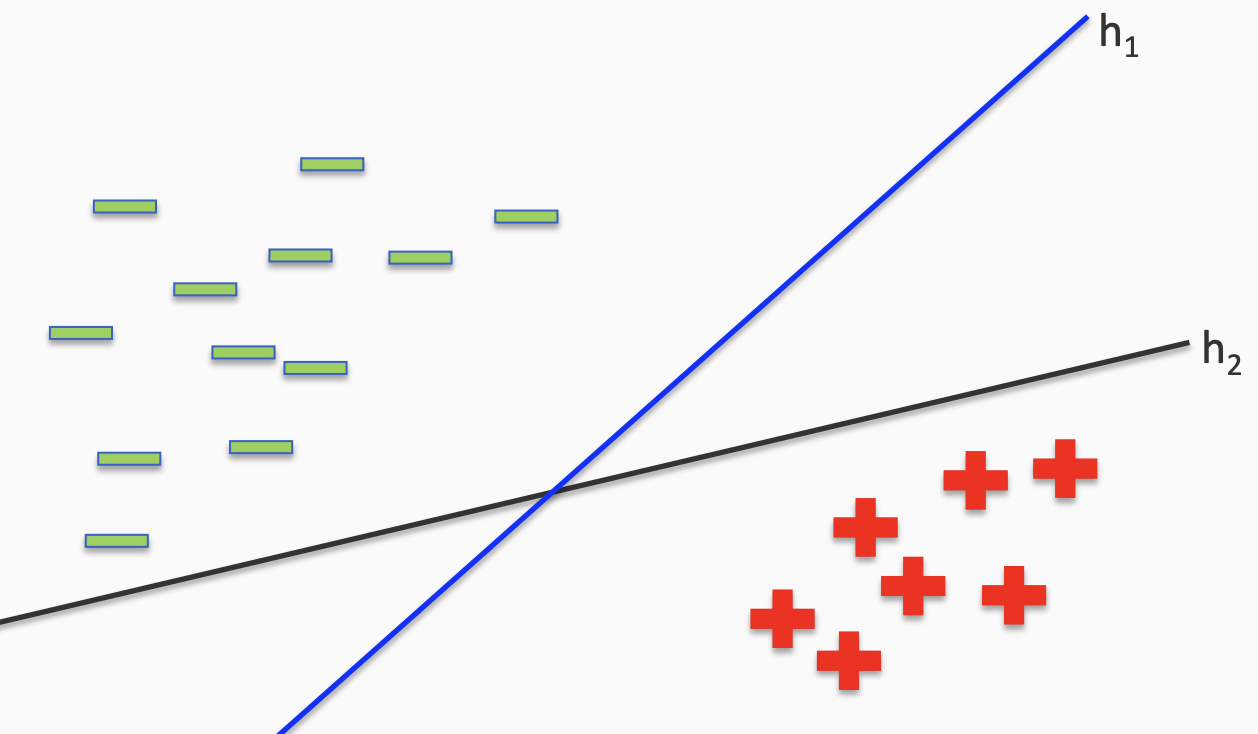
\includegraphics[width=0.5\textwidth]{figures/perceptron_margin}
    \end{figure}
    \fillwithlines{2em}
    \begin{soln}
    Here is a brief algorithm:
    \begin{itemize}
        \item We would first normalize the input samples. Initialize $\mathbf{w}_1=\mathbf{y} \mathbf{x}$, where $\mathbf{x}$ is the first example seen and initialize $t$ to 1.
        \item Predict positive if $\frac{\mathbf{w}_t \cdot \mathbf{x}}{\left\|\mathbf{w}_t\right\|} \geq \gamma / 2$, predict negative if $\frac{\mathbf{w}_t \cdot \mathbf{x}}{\left\|\mathbf{w}_t\right\|} \leq-\gamma / 2$, and consider an example to be a margin mistake when $\frac{\mathbf{w}_t \cdot x}{\left\|\mathbf{w}_t\right\|} \in(-\gamma / 2, \gamma / 2)$.
        \item On a mistake (incorrect prediction or margin mistake), update as in the standard Perceptron algorithm: $\mathbf{w}_{t+1} \leftarrow \mathbf{w}_t+\mathbf{y} \mathbf{x} ; t \leftarrow t+1$.
    \end{itemize}
    \end{soln}   
    \begin{qauthor}
    Varsha, If the students come up with the second and third parts to some extent, we can give them complete credit.
    \end{qauthor}

    \begin{qtester}
   This may be a little difficult. We do not talk about margins much until SVMs. I don't think this was covered with Perceptron. Which learning objective is this addressing?
    \end{qtester}

    \part In this question you will have to answer some questions regarding the perceptron algorithm.
    \begin{subparts}
    \subpart[1] \textbf{Short Answer: }Consider a supervised learning problem with N examples, each of which is a point in d-dimensional space. Let us say our perceptron has converged after t iterations. What is the runtime complexity of the algorithm as a function of N, d, and t? Give a brief explanation of your answer.
    \fillwithlines{1em}
    \begin{soln}
         O(N * d * t), t iterations, each iteration we would perform a dot product which takes O(d) for N samples.
    \end{soln}
    \begin{qauthor}
    Varsha, Implement the perceptron algorithm for binary classification
    \end{qauthor}

    \subpart[2]\textbf{Short Answer: }Let us say we have a learning problem where each input is of d dimensions. Each of these d feature values can only take values 0 or 1. Design a perceptron which classifies the samples as positive if the number of 1s in the feature values of the input is more than the number of 0s. 
    
    \fillwithlines{1em}
    \begin{soln}
         We can have a perceptron where all the weights for d features is 1, and bias term is ceil(-(d+1)/2). (We can get this solution algebraically)
    \end{soln}
    \begin{qauthor}
    Varsha
    \end{qauthor}
    \end{subparts}
\end{parts}

\subsection{Linear Regression}
\begin{parts}

\part[2] \textbf{Numerical answer:} For a linear regression model assume the learning rate $\alpha$ is $0.1$ and the initial value of parameters $\theta_0$ is $0$ and $\theta_1$ is $1$. The training set has 3 samples with the following values:
\begin{center}
    \begin{tabular}{c|c}
		\hline
		x_1& y\\
	    \hline
		1&3 \\
  		3&5 \\
            4&8 \\
		\hline
    \end{tabular}
\end{center}

Use the gradient descent update rule to find the value of parameter $\theta_1$ after one iteration. 
    \begin{tcolorbox}[fit,height=1cm, width=2cm, blank, borderline={1pt}{-2pt}]
    %solution
    \end{tcolorbox}
    \begin{soln}
    1.8
    \end{soln}
    \begin{qauthor}
    Kushagra Agarwal, Implement learning for Linear Regression using ONE optimization technique:(2) gradient descent (the others are saved for Exam 2).
    \end{qauthor}

\part[2] \textbf{Numerical answer:} Suppose you have a quadratic function  $f(x) = 6x^2 - 3x + 5$ that you want to minimize using gradient descent. Apply the gradient descent algorithm with a learning rate $\alpha$ of $0.1$, starting from an initial guess $x=2$ and calculate the new value of $x$ after one iteration.
    \begin{tcolorbox}[fit,height=1cm, width=2cm, blank, borderline={1pt}{-2pt}]
    %solution
    \end{tcolorbox}
    \begin{soln}
    $-0.1$
    \end{soln}
    \begin{qauthor}
    Kushagra Agarwal, Apply gradient descent to optimize a function
    \end{qauthor}
    
\part Suppose that we are an adversary that wants to do \textit{as poorly as possible} on some decision task. This logic has applications to fields such as robust and fair ML, where developers must consider the worst-case performance of their model over a set of plausible distributions of individuals. However, rather than investigating worst-case performance over distributions, we consider worst-case performance on a fixed set $X, Y$, over \textbf{model parameters} $\theta$. 

\begin{subparts}
    
    \subpart[2] \textbf{Short answer}: Write the objective function for this new problem setup, using the variables $\theta \in \mathbb{R}^{M}$ to denote the parameter of interest, $\hat{\theta}$ for the estimated solution of interest, and $J$ to represent the (arbitrary) objective function.

    \begin{soln}
    \begin{align*}
        \hat{\theta} = \argmax_{\theta \in \mathbb{R}^M} J(\theta)
    \end{align*}
    \end{soln}
    
    \subpart[2] \textbf{Short answer}: Explain why the use of this objective for linear regression is flawed in an unconstrained optimization setting.
    
    \begin{soln}
        Note that in this setting, we can make $\hat{\theta}$ \textbf{arbitrarily bad} leading to degenerate solutions if no constraints are imposed on its values. For example, you could adversarially set the values within $\theta$ to approach $\pm \inf$, and as you keep shifting $\theta$ to arbitrarily large-magnitude values, your predictions would become arbitrarily farther away from the solutions, meaning finding an argmax could entail $\theta_i = \pm \inf, 0 \leq i \leq M$.
    \end{soln}

    \subpart[2] \textbf{Short answer}: Propose one way we could ameliorate the above problem.

    \begin{soln}
        Imposing constraints on $\hat{\theta}$, e.g. $||\hat{\theta}||_2^2 \leq \epsilon, \epsilon \in \mathbb{R}$, or $|\hat{\theta} - \theta^*| \leq \epsilon$, where $\theta^*$ denotes the value of $\theta$ that minimizes the objective functions (e.g. OLS solution for 'regular' linear regression; we say that the worst-case $\hat{\theta}$ cannot stray too far from a 'good' solution to the optimization problem)
    \end{soln}
\end{subparts}

\begin{qauthor}
    (1) Kevin, (2) objective functions/closed form solutions in OLS
\end{qauthor}

\part[2] \textbf{Short answer}:
    Consider the following loss function $\ell$, which uses the \textit{absolute value} of the residual between a label $Y$ and its estimation $\hat{Y} = \theta X + \theta_0$, where $X$ is a feature vector and $\theta, \theta_0$ represent a learned set of parameters for regression:
    \begin{align*}
        \ell(Y, \hat{Y}) = |Y - \hat{Y}|
    \end{align*}
    We would like to use $\ell$ in place of residual sum of squares (RSS) when identifying loss over a matrix of training data $X$ and labels $Y$ containing $n$ individuals each, e.g.

    \begin{align*}
        L(X, Y) = \frac{1}{n} \sum_{i = 1}^{n} \ell(Y_i, \theta(X_i) + \theta_0)
    \end{align*}
    
    If possible, provide the closed-form solution to an adaptation of linear regression using the sum of absolute values of residuals $\ell$ in place of RSS. If this is not possible, provide a brief justification as to why, and a potential alternative solution.
    
\begin{soln}
    This is not possible, because the loss function is not differentiable w.r.t. $\hat{y}$ and therefore $x$. As a result, the MLE methods that make a closed-form solution for OLS possible are not applicable to $\ell$. Linear programming/algorithmic approaches on the data should still be able to yield an approximate solution, however.
\end{soln}

\begin{qauthor}
    (1) Kevin, (2) importance of differentiable loss functions in developing closed-form sollutions; consideration of algorithmic techniques for optimization
\end{qauthor}

\part[2] \textbf{Select one}: Consider the following methods of determining whether gradient descent for (unconstrained) OLS linear regression has converged yet. Which of the following would not be valid ways of doing so?

\begin{checkboxes}
    \choice stopping once the L2 norm of the gradient w.r.t. the estimated solution $\theta$ is less than some constant $\epsilon$
    \choice stopping after a fixed set of iterations of gradient descent
    \choice stopping once the L2 norm of the solution $\theta$ is less than a threshold $\epsilon$
    \choice stopping once the change in the objective function from one iteration $t$ to the next iteration $t+1$ is less than a threshold $\epsilon$, e.g. $J(\theta_t; X,Y) - J(\theta_{t+1}; X,Y) \leq \epsilon$
\end{checkboxes}

\begin{soln}
    C
\end{soln}

\begin{qauthor}
    (1) Kevin, (2) stopping conditions in gradient descent for OLS
\end{qauthor}

\begin{qauthor}
    (1) Kevin, (2) importance of differentiable loss functions in developing closed-form sollutions; consideration of algorithmic techniques for optimization
\end{qauthor}
\end{parts}

\subsection{Other/Miscellaneous/Multiple Topics}
\begin{parts}


\part[2] \textbf{Select one:} When we train machine learning models, why do we try to minimize the training error instead of directly minimizing the true error?
    \begin{checkboxes}
     \choice It is possible to calculate the true error, but it is very computationally expensive to find it, so we use the training error instead.
     \choice We don't. With a reasonably large dataset, training error and true error are exactly the same thing.
     \choice Determining the true error requires you to have access to a training dataset that contains every single possible input and output to the model.
     \choice Using the training error instead of the true error guarantees that your learning algorithm will converge.
    \end{checkboxes}
    \begin{soln}
    C. You cannot calculate the true error, since you need to have access to every single point in the domain to do so (and also an accurate error metric). 
    \end{soln}
    \begin{qauthor}
    Rohan Chawla, Explain the difference between true error and training error.
    \end{qauthor}

\end{parts}





% \clearpage
\sectionquestion{Working with Data}

\begin{parts}

\part[2] \textbf{Select all that apply:} Suppose you want to predict whether or not Henry will run some ridiculous, over-the-top demonstration in lecture on any given day. Which of the following models could you use for this task? 
    {%
    \checkboxchar{$\Box$} \checkedchar{$\blacksquare$} % change checkbox style locally
    \begin{checkboxes}
        \choice Decision trees
        \choice $k$-NNs
        \choice Perceptrons
        \choice Linear regressors
        \choice None of the above
    \end{checkboxes}
    }
    \begin{soln}
        A, B, C. The task is a classification task so we cannot use linear regression. 
    \end{soln}
    \begin{qauthor}
        Henry
    \end{qauthor}
    
\part[2] \textbf{Select one:} When we train machine learning models, why do we try to minimize the training error instead of directly minimizing the true error?
    \begin{checkboxes}
     \choice It is possible to compute the true error, but it is very computationally expensive, so we use the training error instead.
     \choice Because given a reasonably large training dataset, training error and true error are exactly the same thing.
     \choice Determining the true error requires you to have access to every single possible input and output to the model.
     \choice Using the training error instead of the true error guarantees that your learning algorithm will converge.
    \end{checkboxes}
    \begin{soln}
    C. You cannot calculate the true error, since you need to have access to every single point in the domain to do so (and also an accurate error metric). 
    \end{soln}
    \begin{qauthor}
    Rohan Chawla, Explain the difference between true error and training error.

    Lightly edited by Henry
    \end{qauthor}

\part[2] \textbf{Short answer:} Imagine that the hypothetical instructors of a hypothetical course have hypothetically decided to train a machine learning model to predict a student's final grade. To do so, they gather data from their current cohort of TAs, who all did excellently in previous offerings of \cancel{10-301/601} this hypothetical course. 

In 1-2 concise sentences, describe the primary issue that may occur when using only TA data to train such a model. 
\fillwithlines{9em}
\begin{soln}
    The dataset only contains information about students with good grades so the model may not be able to learn about (or even output) low grades. 
\end{soln}
\begin{qauthor}
    Henry
\end{qauthor}

\begin{comment}
\part Neural wants to train an ML model on a dataset $\mathcal{D}$, but he accidentally duplicates a subset of the training points in $\mathcal{D}$, giving rise to a new dataset, $\mathcal{D}'$! (Assume for $k$-NN that distance ties are broken by majority vote, and that for $k$-NN and decision trees majority vote ties are broken by returning a constant value.)

\begin{subparts}
    \subpart[2] \textbf{Select all that apply:} If Neural duplicates \textit{all} the points on the dataset, which of these models could possibly differ when trained on $\mathcal{D}'$ instead of on $\mathcal{D}$?
    {%
    \checkboxchar{$\Box$} \checkedchar{$\blacksquare$} % change checkbox style locally
    \begin{checkboxes}
        \choice $k$-NN for classification with $k=1$
        \choice Linear regression
        \choice $k$-NN for classification with $k=3$
        \choice Decision tree for classification
        \choice None of the above
    \end{checkboxes}
    
    \begin{soln}
        C.
    \end{soln}
    
    \subpart[2] \textbf{Select all that apply:} If Neural duplicates \textit{only some but not all} (i.e. a \emph{proper} subset) of the points on the dataset, which of these models could possibly differ when trained on $\mathcal{D}'$ instead of $\mathcal{D}$?
    
    \begin{checkboxes}
        \choice k-NN for classification with $k=1$
        \choice Linear regression
        \choice k-NN for classification with $k=3$
        \choice Decision tree for classification
        \choice None of the above
    \end{checkboxes}
    }
    \begin{soln}
        B, C, D.
    \end{soln}
\end{subparts}
\begin{qauthor}
    Chu. Decision trees, k-NN, linear regression. Objectives: Describe a dataset as points in a high dimensional space, and compare models.
\end{qauthor}

\begin{qtester}
EA Feedback: I like this question
\end{qtester}


\part[2] \textbf{Select all that apply:} Neural wants to predict if a student will show up to class given the student's distance from campus and the weather (sunny or rainy). Neural doesn't know which model to use. Which of the following statements are correct?
    {%
    \checkboxchar{$\Box$} \checkedchar{$\blacksquare$} % change checkbox style locally
    \begin{checkboxes}
        \choice Using a decision tree would not be applicable because decision trees cannot work with real-valued features.
        \choice We can use a $1$-NN model for this task but only if we use the Euclidean distance metric.
        %\choice Since linear regression models predict the label of a point based on real-valued features, Neural could use a linear regression model for this task.
        \choice Using a perceptron model here would be reasonable because perceptrons cannot overfit and therefore are suitable for tasks with a small number of data points.
        \choice None of the above
    \end{checkboxes}
    }
\begin{soln}
D.
\end{soln}
\begin{qauthor}
Chu. Decision trees, logistic regression, and perceptron. Identifying inductive biases of ML models.

Edited by Henry: added option B
\end{qauthor}

\begin{qtester}
EA Feedback: I like this question-- I wonder if we want to be even more specific in the options. I am trying to think of edge cases that students could argue... Or we could add a "Justify" option.
\end{qtester}
\end{comment}

\end{parts}
\clearpage
\sectionquestion{Decision Trees}

\begin{parts}
    
    \part You are a Pokemon trainer and you want to be the very best, that no one ever was. Currently, you are traversing the road from Lavender Town to Fuchsia City. During your journey, you have encountered these six Pokemon:
    
    \begin{center}
        \begin{tabular}{ccc | c}
    		\hline
    		Name & Rarity & Type & Caught?\\
    	    \hline
    		Pikachu & Common & Electric & Yes \\
      		Cattiva & Common & Neutral & No\\
    		Sandshrew & Uncommon & Ground & Yes \\ 
    		Dedenne & Uncommon & Fairy & Yes\\
    		Magicarp & Common & Water & No \\
    		Mewtwo & Legendary & Psychic & No \\ 
    		\hline
        \end{tabular}
    \end{center}
    
    \begin{subparts}
        \subpart[2] \textbf{Numerical answer:} Compute the mutual information between the ``Type'' feature and the label ``Caught?''.
        \begin{tcolorbox}[fit,height=1cm, width=2cm, blank, borderline={1pt}{-2pt}]
            %solution
        \end{tcolorbox}
        \begin{soln}
            1
        \end{soln}
        \begin{qauthor}
            Emily Xie, Use effective splitting criteria for Decision Trees and be able to define entropy, conditional entropy, and mutual information / information gain

            Lightly edited by Henry
        \end{qauthor}
        \begin{qtester}
            You cannot get to Cinnabar island by road, you need to surf there. But you can get to Fuchsia City by road.  
        \end{qtester}
            
        \subpart[2] \textbf{Short answer:} In 2-3 concise sentences, briefly explain why ``Type'' would not be a good feature to initially split on.
        \fillwithlines{15em}
        \begin{soln}
            Even though the entropy is high, the model is likely memorizing the label for each type, thus overfitting on type. We would need to catch more Pokemon of the same types to better generalize the decision of this attribute.
        \end{soln}
        \begin{qauthor}
            Emily Xie, Explain the difference between memorization and generalization

            Lightly edited by Henry
        \end{qauthor}
        
        As you continue your journey, you encounter and successfully catch 200 Pokemon all with ``Rarity'' equal to ``Common''. They are evenly distributed over 10 different values for the ``Type'' feature, none of which you observed in your original dataset. 
        
        \subpart[2] \textbf{Select one:} Appending this new data to your original dataset, how will the entropy of the labels $H(\text{Caught?})$ change? 
        \begin{checkboxes}
            \choice $H(\text{Caught?})$ will increase
            \choice $H(\text{Caught?})$ will decrease
            \choice $H(\text{Caught?})$ will stay the same
            \choice $H(\text{Caught?})$ could increase or decrease depending on the data
        \end{checkboxes}
        \begin{soln}
            B. H(caught?) is initially 1 but decreases (significantly) after catching 200 Pokemon
        \end{soln}
        \begin{qauthor}
            Emily Xie, Use effective splitting criteria for Decision Trees and be able to define entropy, conditional entropy, and mutual information / information gain

            Lightly edited by Henry
        \end{qauthor}
        \begin{qtester}
            I agree that H(caught) decreases but can you explain why information is gained? 
    
            Reword beginning to "As you continue your journey, you do not encounter any more legendary types..." because we were already on the road in part a where we did get a legendary    
        \end{qtester}

        \clearpage
        
        \subpart[2] \textbf{Select one:} Appending this new data to your original dataset, how will the mutual information between the ``Rarity'' feature and the label ``Caught?'' change?
        \begin{checkboxes}
            \choice The mutual information will increase
            \choice The mutual information will decrease
            \choice The mutual information will stay the same
            \choice The mutual information could increase or decrease depending on the data
        \end{checkboxes}
        \begin{soln}
            A, if all the additional 200 data points all have ``Rarity'' = ``Common'' and ``Caught?'' = ``Yes'', then the conditional entropy $H(\text{Caught?}\mid \text{Rarity = Common})$ will significantly decrease, the weight on this value in the mutual information will go up and all the other conditional entropies will stay the same; hence the mutual information will increase. 
        \end{soln}
        \begin{qauthor}
            Emily Xie, Use effective splitting criteria for Decision Trees and be able to define entropy, conditional entropy, and mutual information / information gain

            Edited by Henry to ask about Rarity instead of Type; \textbf{Note to the testers}: please double check the logic in this question and that it can reasonably be solved without having to do any math. 
        \end{qauthor}
    
        \begin{qtester}
            Fix formatting of "given"
            
            To answer this I think people need to know how many total "types" of pokemon there are. E.g. if someone thinks there are 100 types, their answer will not be what is intended
        \end{qtester}
    \end{subparts}
    
    \part Younha has trained a decision tree to classify chest x-rays as diseased or non-diseased. After she trains her initial tree on human and monkey x-rays, her friend hands her some mouse x-ray images, which she decides to use as the dataset to prune her tree with. 
    
    \begin{subparts}
        \subpart[2] \textbf{Select one:} Which of the following metrics should she report as the \emph{validation} error rate of her pruned tree?
        \begin{checkboxes}
            \choice The fraction of human x-rays misclassified by her decision tree.
            \choice The fraction of monkey x-rays misclassified by her decision tree.
            \choice The fraction of mouse x-rays misclassified by her decision tree.
            \choice The fraction of all x-rays (human, monkey and mouse combined) misclassified by her decision tree.
        \end{checkboxes}
        \begin{soln}
            C. The validation set is the set that the hyperparameter tuning/pruning process uses, which in this case are the mouse x-rays. As such, the error associated with the mouse x-ray classifications are the validation error she is interested in.
        \end{soln}
        \begin{qtester}
            You marked A but wrote C. 
        \end{qtester}
            
        \subpart[3] \textbf{Short answer:} Younha has a separate dataset of monkey x-rays that she thought were too low quality, so she did not include them while training her tree. Her friend tells her that the images are good enough, so she computes the error rate of her pruned decision tree on this dataset. 
        
        However, since she included monkey x-rays in her original training dataset, she is worried that this metric is overly optimistic i.e., the error rate she computed is lower than the true error of her pruned tree on \emph{similar, low quality monkey x-rays}. Do you agree with her conclusion? Briefly justify your answer in 1-2 concise sentences.
        \fillwithlines{9em}
        \begin{soln}
            No, this test error rate is unbiased: even though her training data included monkey images, the ``lower quality'' images weren't part of that dataset, so her metric shouldn't be overly optimistic.
        \end{soln}   
    \end{subparts}
    \begin{qauthor}
        Andrew, Explain the difference between (1) training error, (2) validation error, (3) cross-validation error, (4) test error, and (5) true error

        Edited by Henry
    \end{qauthor}

    \clearpage
    
    \part For the following questions, consider the training dataset in Figure \ref{fig:neuraldtreedata} consisting of 10 data points, where each point is labeled as either a square $y = \blacksquare$ or a triangle $y = \blacktriangle$.
    
    \begin{figure}[h]
        \begin{center}
            \begin{tikzpicture}
            \begin{axis}[
                scale=0.9, width=10cm, height=10cm, mark options={scale=1.7},
                xmin=0, xmax=9, xtick={1,2,3,4,5,6,7,8},
                ymin=0, ymax=9, ytick={1,2,3,4,5,6,7,8},
                samples=50, xlabel=$x_1$, ylabel=$x_2$]]
                \addplot [
                    scatter,
                    only marks,
                    point meta=explicit symbolic,
                    scatter/classes={
                        a={mark=triangle*,red},
                        b={mark=square*,blue}
                    },
                    nodes near coords*={},
                    visualization depends on={\thisrow{myvalue} \as \myvalue},
                ] table [meta=label] {
                    x y label myvalue
                    2 1 a 1
                    4 2 a 1
                    6 1 a 1
                    1 5 b 1
                    5 5 b 1
                    6 6 b 1
                    3 8 b 1
                    5 8 b 1
                    7 8 a 1
                    8 8 a 1
                };
            \end{axis}
            \end{tikzpicture} 
        \end{center}
        \caption{}
        \label{fig:neuraldtreedata}
    \end{figure}
    
    \begin{subparts}
        \subpart[3] \textbf{Fill in the blank:} Complete the decision tree in Figure \ref{fig:neuraldtree} by filling in each of the blanks in the diagram such that the final tree achieves zero training error on the dataset shown in Figure \ref{fig:neuraldtreedata}.

        \begin{figure}[h!]
            \def\splitDist{5cm}
            \def\rootDist{4cm}
            \centering
            \begin{tikzpicture}[
                    scale=0.75,
                    node/.style = {draw, rectangle},
                    oval/.style = {ellipse, draw, inner xsep=#1},
                    > = stealth, % arrow head style
                    shorten > = 0pt, % don't touch arrow head to node
                    auto,
                    thick % line style
                ]
        
                \node[node, text height=1cm, minimum height=1.2cm, minimum width=4cm] (S1) {$x_2 \textrm{\quad \underline{\quad \quad \quad} \quad} 7$};
                \path (S1) ++(-135:\splitDist) node [node, text height=1cm, minimum height=1.5cm, minimum width=4cm] (S2) {$x_1 \textrm{\quad $<$ \quad \underline{\quad \quad \quad} \quad}$};
                \path (S1) ++(-45:\splitDist) node [node, text height=1cm, minimum height=1.5cm, minimum width=4cm] (S3) {$x_2 \textrm{\quad $>$ \quad \underline{\quad \quad \quad} \quad}$};
                \path (S2) ++(-135:\rootDist) node [oval] (L1) {$\blacksquare$};
                \path (S2) ++(-45:\rootDist) node [oval] (L2) {$\blacktriangle$};
                \path (S3) ++(-135:\rootDist) node [oval] (L3) {$\blacksquare$};
                \path (S3) ++(-45:\rootDist) node [oval] (L4) {$\blacktriangle$};
            
                \draw (S1) -- (S2) node [left,pos=0.25] {true \quad};
                \draw (S1) -- (S3) node [right,pos=0.25] {\quad false};
                \draw (S2) -- (L1) node [left,pos=0.25] {true \quad};
                \draw (S2) -- (L2) node [right,pos=0.25] {\quad false};
                \draw (S3) -- (L3) node [left,pos=0.25] {true \quad};
                \draw (S3) -- (L4) node [right,pos=0.25] {\quad false};
            \end{tikzpicture}
            \caption{}
            \label{fig:neuraldtree}
        \end{figure}

        \subpart[3] \textbf{Drawing:} On Figure \ref{fig:neuraldtreedata}, draw the decision boundary corresponding to your decision tree from the previous question. For full credit, you must shade in the region(s) labeled as $y=\blacksquare$.
    \end{subparts}
    
    \begin{soln}
        The first blank must be $>$. The left blank must be in $(5, 7]$ and the right blank must be in $[2, 5)$. Here is one possible answer (arguably the most reasonable one) and the corresponding decision boundary:
    
        \begin{figure}[h!]
            \def\splitDist{5cm}
            \def\rootDist{4cm}
            \centering
            \begin{tikzpicture}[
                    scale=0.8,
                    node/.style = {draw, rectangle},
                    oval/.style = {ellipse, draw, inner xsep=#1},
                    > = stealth, % arrow head style
                    shorten > = 0pt, % don't touch arrow head to node
                    auto,
                    thick % line style
                ]
        
                \node[node, text height=1cm, minimum height=1.5cm, minimum width=4cm] (S1) {$x_2 > 7$};
                \path (S1) ++(-135:\splitDist) node [node, text height=1cm, minimum height=1.5cm, minimum width=4cm] (S2) {$x_1 \textrm{\quad $<$ \quad \underline{6} \quad}$};
                \path (S1) ++(-45:\splitDist) node [node, text height=1cm, minimum height=1.5cm, minimum width=4cm] (S3) {$x_2 \textrm{\quad $>$ \quad \underline{3} \quad}$};
                \path (S2) ++(-135:\rootDist) node [oval] (L1) {$\blacksquare$};
                \path (S2) ++(-45:\rootDist) node [oval] (L2) {$\blacktriangle$};
                \path (S3) ++(-135:\rootDist) node [oval] (L3) {$\blacksquare$};
                \path (S3) ++(-45:\rootDist) node [oval] (L4) {$\blacktriangle$};
            
                \draw (S1) -- (S2) node [left,pos=0.25] {true \quad};
                \draw (S1) -- (S3) node [right,pos=0.25] {\quad false};
                \draw (S2) -- (L1) node [left,pos=0.25] {true \quad};
                \draw (S2) -- (L2) node [right,pos=0.25] {\quad false};
                \draw (S3) -- (L3) node [left,pos=0.25] {true \quad};
                \draw (S3) -- (L4) node [right,pos=0.25] {\quad false};
            \end{tikzpicture}
            \caption{}
            \label{fig:neuraldtree}
        \end{figure}
        
        \begin{center}
            \begin{tikzpicture}
            \begin{axis}[
                scale=0.9, width=10cm, height=10cm, mark options={scale=1.7},
                xmin=0, xmax=9, xtick={1,2,3,4,5,6,7,8},
                ymin=0, ymax=9, ytick={1,2,3,4,5,6,7,8},
                samples=50, xlabel=$x_1$, ylabel=$x_2$]]
                \addplot[red, ultra thick, dotted] coordinates { (0,3) (9,3) };
                \addplot[red, ultra thick, dotted] coordinates { (0,7) (9,7) };
                \addplot[red, ultra thick, dotted] coordinates { (6,7) (6,9) };
                \addplot[fill=blue, fill opacity=0.1] coordinates { (0, 3.01) (9, 3.01) (9, 6.99) (5.99, 6.99) (5.99, 9) (0, 9) (0, 3.01) } \closedcycle;
                \addplot [
                    scatter,
                    only marks,
                    point meta=explicit symbolic,
                    scatter/classes={
                        a={mark=triangle*,red},
                        b={mark=square*,blue}
                    },
                    nodes near coords*={},
                    visualization depends on={\thisrow{myvalue} \as \myvalue},
                ] table [meta=label] {
                    x y label myvalue
                    2 1 a 1
                    4 2 a 1
                    6 1 a 1
                    1 5 b 1
                    5 5 b 1
                    6 6 b 1
                    3 8 b 1
                    5 8 b 1
                    7 8 a 1
                    8 8 a 1
                };
            \end{axis}
            \end{tikzpicture} 
        \end{center}
    \end{soln}
    \begin{qauthor}
        Henry
    \end{qauthor}
    
    \part[3] \textbf{Fill in the blank:} Complete the following paragraph about training decision trees by circling the best of the provided options for each of blanks: 
    
    \doublespacing
    \begin{quote}
            Paloma the Possum is training a decision tree and notices that there is a \underline{\quad large \quad / \quad small \quad} difference between her training and test error rates, a classic sign of overfitting. 
            
            She suspects this is because the maximum depth that she allowed her decision tree to grow to, a model \underline{\quad parameter \quad / \quad hyperparameter \quad}, was too \underline{\quad large \quad / \quad small \quad}.
    \end{quote}
    \singlespacing
    
    \begin{soln}
        Paloma the Possum is training a decision tree and notices that there is a large difference between her training and test error rates, a classic sign of overfitting. She suspects this is because the maximum depth that she allowed her decision tree to grow to, a model hyperparameter, was too large.
    \end{soln}
    \begin{qauthor}
        Bhargav, Judge whether a decision tree is "underfitting" or "overfitting", Plan an experiment that uses training, validation, and test datasets to predict the performance of a classifier on unseen data (without cheating)

        Edited by Henry
    \end{qauthor}
    
\end{parts}

\clearpage
\sectionquestion{k-Nearest Neighbors}

\begin{parts}
\part You are given a training dataset containing information about various species of strawberries. Each species is described by its weight (in grams) and its sweetness (on a scale from 0 to 5). You want to use $k$-NN to classify which species are popular. You create a binary classification task by assigning a species a label of $+$ if the species is popular and $-$ otherwise. Consider the following dataset:
\begin{align*}
    D &= \{(x^{(i)}, y^{(i)})\}_{i=1}^{7}\\
    &= \{((1,4),+),((2,1),-),((2,4), +), ((3,2), -),((3,3),-),((4,1),+),((4,4),+)\}
\end{align*}
where $\xv^{(i)} \in \mathbb{R}^{2} = (\text{weight}, \text{sweetness})$ and $y^{(i)} \in \{+, -\}$ is the label.

For your convenience, we've plotted this dataset in the figure below:

\begin{center}
    \begin{tikzpicture}
        \begin{axis}[
            scale=1.5, axis equal image, mark options={scale=1.5},
            xmin=0, xmax=5, xtick={1,...,4},
            ymin=0, ymax=5, ytick={1,...,4},
            samples=50, grid=major, xlabel=Weight, ylabel=Sweetness]]
            \addplot [
                scatter,
                only marks,
                point meta=explicit symbolic,
                scatter/classes={
                    a={mark= +,blue},
                    b={mark= -,red}
                },
                nodes near coords*={$\xv^{(\pgfmathprintnumber[frac]\myvalue)}$},
                visualization depends on={\thisrow{myvalue} \as \myvalue},
            ] table [meta=label] {
                x y label myvalue
                1 4 a 1
                2 1 b 2
                2 4 a 3
                3 2 b 4
                3 3 b 5
                4 1 a 6
                4 4 a 7
            };
        \end{axis}
    \end{tikzpicture}   
\end{center}
        
You fit a $k$-NN model to this training dataset using the Euclidean distance. When computing the nearest neighbors, if two points are equally close to some input, ties are broken by selecting the less sweet species; if the two points are equally sweet, we break ties in favor of the less heavy species. % (Example tie scenario: if $k=2$, $(1,3)$ and $(3,3)$ have the same euclidean distance with $(2,3)$, then we choose $(1,3)$ as the closest point.)

\begin{subparts}
    \begin{comment}
    \subpart[2] \textbf{Drawing:} Given the training dataset shown above, plot each data point in the graph below by drawing its label, either a $+$ or a $-$, in the correct location:

    \begin{center}
        \begin{tikzpicture}
        \begin{axis}[
            scale=1.5, axis equal image, mark options={scale=1.5},
            xmin=0, xmax=6, xtick={1,...,5},
            ymin=0, ymax=6, ytick={1,...,5},
            samples=50, grid=major, xlabel= Weight, ylabel=Sweetness]]
        \end{axis}
        \end{tikzpicture} 
    \end{center}
    \end{comment}

    \subpart[4] \textbf{Drawing:} On the figure provided above, draw the decision boundary for a $1$-NN model.
    
    \begin{soln}
        \begin{center}
        \begin{tikzpicture}
        \begin{axis}[
            scale=1.5, axis equal image, mark options={scale=1.5},
            xmin=0, xmax=5, xtick={1,...,4},
            ymin=0, ymax=5, ytick={1,...,4},
            samples=50, grid=major, xlabel=Weight, ylabel=Sweetness]]
            \addplot[red, ultra thick, dotted] coordinates { (0, 2) (1.5, 2.5) };
            \addplot[red, ultra thick, dotted] coordinates { (1.5, 2.5) (3, 4) };
            \addplot[red, ultra thick, dotted] coordinates { (3, 4) (4.5, 2.5) };
            \addplot[red, ultra thick, dotted] coordinates { (4.5, 2.5) (2, 0)};
            \addplot [
                scatter,
                only marks,
                point meta=explicit symbolic,
                scatter/classes={
                    a={mark= +,red},
                    b={mark= -,red}
                },
                nodes near coords*={$\xv^{(\pgfmathprintnumber[frac]\myvalue)}$},
                visualization depends on={\thisrow{myvalue} \as \myvalue},
            ] table [meta=label] {
                x y label myvalue
                1 4 a 1
                2 1 b 2
                2 4 a 3
                3 2 b 4
                3 3 b 5
                4 1 a 6
                4 4 a 7
            };
        \end{axis}
        \end{tikzpicture}   
        \end{center}
    \end{soln}
    \begin{qauthor}
        Zoe Xu, Describe a dataset as points in a high dimensional space
    
        Edited by Henry
    \end{qauthor}
    
    \subpart[2] \textbf{Numerical answer:} What is the training error of a $3$-NN on this dataset? \textbf{Report your answer as a fraction.}
    \begin{tcolorbox}[fit,height=1cm, width=2cm, blank, borderline={1pt}{-2pt}]
    %solution
    \end{tcolorbox}
    \begin{soln}
        $\frac{1}{7}$; I believe the only incorrectly predicted data point is $x^{(6)}$
    \end{soln}
    \begin{qauthor}
        Zoe Xu, implement $k$-NN algorithm and deal with tie scenario.

        Edited by Henry 
    \end{qauthor}

\begin{qtester}
    Should this be 3/7? x1, x7, x6?
    
    Zoe: Yes! Thank you very much. I should look at the answer more carefully.
\end{qtester}
    
    \subpart[2] \textbf{Select all that apply:} Let's say we have a new species with weight 1 and sweetness 3, and the new species is \textbf{not} popular among the market. For which values of $k$ is this new species correctly classified by a $k$-NN classifier?
    {
    \checkboxchar{$\Box$} \checkedchar{$\blacksquare$} % change checkbox style locally
    \begin{checkboxes}
     \choice $k = 1$
     \choice $k = 3$
     \choice $k = 5$
     \choice $k = 7$
     \choice None of the above
    \end{checkboxes}
    }
    \begin{soln}
    $C$
    \end{soln}
    \begin{qauthor}
        Zoe Xu, implement $k$-NN algorithm and deal with tie scenario.

        Edited by Henry
    \end{qauthor}
    \begin{qtester}
    At this point we are testing, so k=1 should not be valid right? 

    Zoe Xu: Yes! You're right. Thanks again!s
    \end{qtester}

    \subpart[2] \textbf{Short answer:} Looking at the training errors for different values of $k$, you choose the model with $k = 1$ as it has the lowest training error. Do you think this approach will lead to good performance on a held-out test dataset? If you answered yes, briefly justify your answer and if you answered no, briefly describe an alternative method that you think would lead to better performance; limit your response to 1-2 concise sentences. 
    
    \fillwithlines{9em}
    \begin{soln}
    No, we would use validation dataset (validation error) to choose k as k is a hyperparameter.
    \end{soln}
    \begin{qauthor}
        Zoe Xu (citing from practice problem Exam1 F23), one point for true or false, and one point for reason.
        Describe the inductive bias of a $k$-NN classifier
    \end{qauthor}

\end{subparts}

\part[2] \textbf{Select all that apply:} Which of the following statement(s) about $k$-NNs is/are true? % Assume a point can be its own neighbor.
    {%
    \checkboxchar{$\Box$} \checkedchar{$\blacksquare$} % change checkbox style locally
    \begin{checkboxes}
     \choice $k$-NN can be applied to classification problems but not regression problems.
     \choice We can always achieve zero training error with a $1$-NN model, but it may not generalize well in testing.
     \choice Decreasing $k$ can help address overfitting.
     \choice Computing the predictions of a $k$-NN model becomes more computationally expensive as the number of features grows. 
     \choice None of the above
    \end{checkboxes}
    }
    \begin{soln}
    $B, D$
    \end{soln}
    \begin{qauthor}
        Zoe Xu, test understanding of $k$-NN model
    \end{qauthor}

\clearpage

    \part[2] \textbf{Short Answer:} Suppose we have a binary classification task where the labels are coded as $y\in \{-1,+1\}$. We create the following variant of the $k$-NN classifer with $k=4$ that uses the Euclidean distance metric: $h(\xv') = \hat{y}' = \textrm{sign}(2y_1 + y_2 + y_3 + y_4)$, where $y_i$ is the label of the $i$-th closest point to $\xv'$ ($i = 1, 2, \cdots, 4$). Assume that there are at least $4$ data points in the training dataset. 
    
    Essentially, our model assigns double the weight to the closest point relative to the three other nearest neighbors. If there is a tie for the closest point to $\xv'$, then we choose an arbitrary point to get double the vote. Your friend claims that ties in the vote will never happen (i.e, the value inside the sign expression will never be $0$). Is your friend correct? Briefly justify your answer in 2-3 concise sentences. 
    \fillwithlines{15em}
    \begin{soln}
    Your friend is correct. Since each point is classified as +1 or -1, with three points, the only possible values for the sum are $\{-5, -4, -3, -1, 1, 3, 4, 5\}$. The value for the closest point is either +2 or -2, which means that if we add the values of all the points with the weights, we will never get 0.
    \end{soln}
    \begin{qauthor}
    Bhargav, Invent "new" k-NN learning algorithms capable of dealing with even k
    \end{qauthor}

\part[2] Suppose you train a $k$-NN classifier using Euclidean distance on \emph{binary} vectors $\x$ of length $D$, i.e., the value of each feature is either $0$ or $1$. Unfortunately, you find that the performance of your classifier on some held out test dataset $\mathcal{D}_{\textrm{test}}$ isn't very good. 

\textbf{True or False:} Switching from the Euclidean distance to the Manhattan distance \emph{could} improve the performance of your classifier on $\mathcal{D}_{\textrm{test}}$. Briefly justify your answer in 1-2 concise sentences. Recall that the Manhattan distance between vectors is: 
    
    \[d(\x,\x') = \sum_{i=1}^D |x_i-x_i'|\]
    
    \begin{checkboxes}
        \choice True
        \choice False
    \end{checkboxes}
    \fillwithlines{9em}
    \begin{soln}
        False; the Euclidean distance and Manhattan distance will behave identically on binary vectors in terms of determining relative distances between points. 
    \end{soln}

\end{parts}
% \sectionquestion{k-Nearest Neighbors}

\begin{parts}



\part Let's revisit the task of predicting whether or not someone will be diagnosed with heart disease. Recall in lecture we based our predictions on three categorical features:
\begin{enumerate}
    \item Family History ($F$): \{Yes, No\}
    \item Cholesterol ($C$): \{Normal, Abnormal\}
    \item Blood Pressure ($B$): \{Low, Medium, High\}
\end{enumerate}
Let's apply a $k$-NN model to this problem! In order to do so, we'll use the following distance metric:
\[
    d(\x, \x') = \sum_{i \in \{F, C, B\}} d_i(x_i, x_i')
\]
where $d_F$, $d_C$ and $d_B$ are distance metrics over each feature, which can be defined by enumerating every possible pair of values: 

\begin{table}[h!]
    \begin{subtable}[c]{0.2\textwidth}
        \centering
        \begin{tabular}{c|c|c|}
            & Yes & No \\ \hline
            Yes & $0$ & $1$ \\ \hline
            No & $1$ & $0$ \\ \hline
        \end{tabular}
        \subcaption*{\large $d_F$}
    \end{subtable}
    \begin{subtable}[c]{0.4\textwidth}
        \centering
        \begin{tabular}{c|c|c|}
            & Normal & Abnormal \\ \hline
            Normal & $0$ & $1$ \\ \hline
            Abnormal & $1$ & $0$ \\ \hline
        \end{tabular}
        \subcaption*{\large $d_C$}
    \end{subtable}
    \begin{subtable}[c]{0.4\textwidth}
        \centering
        \begin{tabular}{c|c|c|c|}
            & Low & Medium & High \\ \hline
            Low & $0$ & $1$ & $2$ \\ \hline
            Medium & $1$ & $0$ & $1$ \\ \hline
            High & $2$ & $1$ & $0$ \\ \hline
        \end{tabular}
        \caption*{\large $d_B$}
    \end{subtable}
\end{table}

To answer the following questions, let $\x' = [F=$ Yes, $C=$ Normal, $B=$ High$]$ be a new patient we are interested in making a prediction for. We will use this training dataset:

\begin{table}[h!]
    \centering
    \begin{tabular}{c|c|c|c}
        $F$ & $C$ & $B$ & $Y$ \\ \hline
        Yes & Normal & Low & No Heart Disease \\ \hline
        No & Abnormal & Low & No Heart Disease \\ \hline
        Yes & Abnormal & High & Heart Disease \\ \hline
        Yes & Abnormal & Medium & No Heart Disease \\ \hline
        No & Abnormal & Medium & Heart Disease \\ \hline
        No & Normal & Low & Heart Disease \\ \hline
    \end{tabular}
\end{table}

\begin{comment}
\begin{table}[h!]
    \centering
    \begin{tabular}{c|c|c|c|c|c}
        $i$ & $F$ & $C$ & $B$ & $Y$ & $d(\x^{(i)}, \x')$ \\ \hline
        1 & Yes & Normal & Low & No Heart Disease & 2 \\ \hline
        2 & No & Abnormal & Low & No Heart Disease & 4 \\ \hline
        3 & Yes & Abnormal & High & Heart Disease & 1 \\ \hline
        4 & Yes & Abnormal & Medium & No Heart Disease & 2 \\ \hline
        5 & No & Abnormal & Medium & Heart Disease & 3 \\ \hline
        6 & No & Normal & Low & Heart Disease & 3 \\ \hline
    \end{tabular}
\end{table}

Note that we have precomputed the distances between $\x'$ and all the training data points in the last column of the table above. 
\end{comment}

\begin{subparts}
    \subpart[1] \textbf{Select one:} What would a 1-NN model predict as the label for $\x'$?
    \begin{checkboxes}
        \choice Heart Disease
        \choice No Heart Disease
    \end{checkboxes}
    \begin{soln}
        Heart Disease
    \end{soln}
    
    \subpart[2] \textbf{Select one:} What would a 3-NN model predict as the label for $\x'$?
    \begin{checkboxes}
        \choice Heart Disease
        \choice No Heart Disease
    \end{checkboxes}
    \begin{soln}
        No Heart Disease
    \end{soln}

    \clearpage
    
\begin{EnvFullwidth}    
Now suppose you decide that patients with Normal and Abnormal cholesterol are fundamentally different and you define a new distance metric, $d_C^{(\textrm{new})}$ to reflect this:
\end{EnvFullwidth}

\begin{table}[h!]
    \centering
    \begin{tabular}{c|c|c|}
        & Normal & Abnormal \\ \hline
        Normal & $0$ & $1000$ \\ \hline
        Abnormal & $1000$ & $0$ \\ \hline
    \end{tabular}
    \caption*{\large $d_C^{(\textrm{new})}$}
\end{table}
    
    \subpart[1] \textbf{Select one:} Using $d_C^{(\textrm{new})}$ instead of $d_C$ and using the original $d_F$ and $d_B$, what would a 1-NN model predict as the label for $\x'$?
    \begin{checkboxes}
        \choice Heart Disease
        \choice No Heart Disease
    \end{checkboxes}
    \begin{soln}
        No Heart Disease
    \end{soln}
    
    \subpart[2] \textbf{Select one:} Using $d_C^{(\textrm{new})}$ instead of $d_C$ and using the original $d_F$ and $d_B$, what would a 3-NN model predict as the label for $\x'$?
    \begin{checkboxes}
        \choice Heart Disease
        \choice No Heart Disease
    \end{checkboxes}
    \begin{soln}
        Heart Disease
    \end{soln}
    
\begin{EnvFullwidth} 
In order to choose between $d_C$ and $d_C^{(\textrm{new})}$, you gather a validation dataset and compare the performance of two 3-NN models on this dataset, one that uses $d_C$ and one that uses $d_C^{(\textrm{new})}$. You find that the 3-NN model that uses $d_C^{(\textrm{new})}$ achieves a lower validation error rate. 
\end{EnvFullwidth}

    \subpart[2] \textbf{True or False:} Because you did not use the validation dataset to pick what value of $k$ to use, the validation error rate of the 3-NN model that uses $d_C^{(\textrm{new})}$ is a good estimate of that model's true error rate. \textbf{Briefly justify your answer in 1 concise sentence.}
    \begin{checkboxes}
        \choice True
        \choice False
    \end{checkboxes}
    \fillwithlines{6em}
    \begin{soln}
        False: the validation dataset was used to pick between models, it will be overly optimistic about the performance of the better of the two models. Put differently, model selection is equivalent to hyperparameter optimization and as such, we need a held-out test dataset to evaluate the test error rate. 
    \end{soln}
        
\clearpage

\begin{EnvFullwidth}    
    After making the change above, you decide that you like this new distance metric better and you should scale the other distance metrics, $d_F$ and $d_B$, by $1000$ as well, giving rise to $d_F^{(\textrm{new})}$ and $d_B^{(\textrm{new})}$. You use these to define a new distance metric:
    \[
        d^{(\textrm{new})}(\x, \x') = \sum_{i \in \{F, C, B\}} d_i^{(\textrm{new})}(x_i, x_i')
    \]
\end{EnvFullwidth}

    \subpart[2] \textbf{True or False:} a $k$-NN model using $d$ as a distance metric will make the exact same predictions as a $k$-NN model using $d^{(\textrm{new})}$ $\forall$ values of $k$. \textbf{Briefly justify your answer in 1-2 concise sentences.}
    \begin{checkboxes}
        \choice True
        \choice False
    \end{checkboxes}
    \fillwithlines{6em}
    \begin{soln}
        True, scaling each feature-wise distance only changes the magnitude of the overall distances, not the relative ranking of all training data points by distance with a particular $\x'$.
        
        True, the distances are all scaled proportionally such that for each point the set of nearest neighbors does not change.
    \end{soln}
\end{subparts}
\begin{qauthor}   
    Henry; AUTHOR'S NOTE: a previous version of this question included the precomputed distances between $\x'$ and each data point (see the commented out portion). Testers please comment on whether or not you think this should be included. 
\end{qauthor}

\part[4] \textbf{Fill in the blanks:} Neural the Narwhal gathers a training dataset consisting of 5 one-dimensional examples and builds three $k$-NN models: one with $k=1$, one with $k=3$ and one with $k=5$; all models use Euclidean distance. He sends you the training error rates for each model along with the actual dataset but unfortunately, some of the data is corrupted and you only receive the following information.

\begingroup
\renewcommand{\arraystretch}{2}
\begin{center}
\begin{tabular}{cc}
    \begin{tabular}{c|c|c}
    $i$ & $x^{(i)}$ & $y^{(i)}$ \\ \hline
    1 & 2 & $+1$ \\ 
    2 & 4 & $-1$ \\ 
    3 & 7 & $+1$ \\ 
    4 & 8 & \underline{\qquad\qquad} \\ 
    5 & 9 & \underline{\qquad\qquad} \\ 
    \end{tabular} 
    &
    \begin{tabular}{c|c}
    $k$ & training error rate \\ \hline
    1 & \underline{\qquad\qquad} \\ 
    3 & 0.2 \\ 
    5 & \underline{\qquad\qquad}
    \end{tabular}
\end{tabular}
\end{center}
\endgroup

In the spaces provided above, fill in all missing fields (i.e., the training error rates for the $1$-NN and $5$-NN models as well as the labels $y^{(4)}$ and $y^{(5)}$); if you do not have enough information to deduce a missing value, write ``?'' in the space provided. 

\begin{soln}
    $y^{(4)}=y^{(5)}=+1$, the training error of the $1$-NN model is 0 (always) and the training error of the $5$-NN model is 0.2. 
    
    Based on the $3$-NN training error rate, we know that it only makes 1 mistake. $x^{(2)}$ is already misclassified so $x^{(4)}$ and $x^{(5)}$ must both be correctly classified by the $3$-NN model, which only occurs if both $y^{(4)}$ and $y^{(5)}$ are $+1$. Finally the $5$-NN model or majority vote would classify everything as $+1$, making one mistake so it also has a training error rate of 0.2. 
\end{soln}
\begin{qauthor}
    Henry
\end{qauthor}

\clearpage

\begin{comment}
\part[2] Suppose you train a $k$-NN classifier using Euclidean distance on \emph{binary} vectors $\x$ of length $D$, i.e., the value of each feature is either $0$ or $1$. Unfortunately, you find that the performance of your classifier on some held out test dataset $\mathcal{D}_{\textrm{test}}$ isn't very good. 

\textbf{True or False:} Switching from the Euclidean distance to the Manhattan distance \emph{could} improve the performance of your classifier on $\mathcal{D}_{\textrm{test}}$. \textbf{Briefly justify your answer in 1-2 concise sentences.}  Recall that the Manhattan distance between vectors is: 
    
    \[d(\x,\x') = \sum_{i=1}^D |x_i-x_i'|\]
    
    \begin{checkboxes}
        \choice True
        \choice False
    \end{checkboxes}
    \fillwithlines{6em}
    \begin{soln}
        False; the Euclidean distance and Manhattan distance will behave identically on binary vectors in terms of determining relative distances between points. 
    \end{soln}

    \subpart[2] \textbf{True or False:} Switching from $k = 3$ to $k = 1$ \emph{could} improve the performance of your classifier on $\mathcal{D}_{\textrm{test}}$. \textbf{Briefly justify your answer in 1-2 concise sentences.}
    
    \begin{checkboxes}
        \choice True
        \choice False
    \end{checkboxes}
    \fillwithlines{6em}
    \begin{soln}
        True; this depends on the labels of the test and training datasets but is absolutely possible (it's a bit hard to defend this statement so we should be generous in what justifications we accept).  
    \end{soln}
\end{comment}

\begin{qauthor}
    Henry
\end{qauthor}

\part[3] \textbf{Drawing:} Given the training dataset shown below where each point is labeled as a square $y = \blacksquare$ or a triangle $y = \blacktriangle$,
%squares have label $y=+1$ and red triangles have label $y=-1$,
draw the decision boundary that a 1-nearest neighbor model with Euclidean distance would learn. For full credit, shade in the region(s) labeled as $y = \blacksquare$.
\begin{center}
    \begin{tikzpicture}
    \begin{axis}[
        scale=1.5, axis equal image, mark options={scale=1.5},
        xmin=0, xmax=6, xtick={1,...,5},
        ymin=0, ymax=6, ytick={1,...,5},
        samples=50, grid=major, xlabel=$x_1$, ylabel=$x_2$]]
        \addplot [
            scatter,
            only marks,
            point meta=explicit symbolic,
            scatter/classes={
                a={mark=square*,blue},
                b={mark=triangle*,red}
            },
            nodes near coords*={$\xv^{(\pgfmathprintnumber[frac]\myvalue)}$},
            visualization depends on={\thisrow{myvalue} \as \myvalue},
        ] table [meta=label] {
            x y label myvalue
            1 4 b 1
            3 2 b 2
            4 1 a 3
            5 4 a 4
        };
    \end{axis}
    \end{tikzpicture} 
\end{center}

\begin{soln}
\begin{center}
    \begin{tikzpicture}
    \begin{axis}[
        scale=1.5, axis equal image, mark options={scale=1.5},
        xmin=0, xmax=6, xtick={1,...,5},
        ymin=0, ymax=6, ytick={1,...,5},
        samples=50, grid=major, xlabel=$x_1$, ylabel=$x_2$]]
        \addplot[red, ultra thick, dotted] coordinates { (2, 0) (4.5, 2.5) };
        \addplot[red, ultra thick, dotted] coordinates { (4.5, 2.5) (3, 4) };
        \addplot[red, ultra thick, dotted] coordinates { (3, 4) (3 ,6) };
        \addplot [
            scatter,
            only marks,
            point meta=explicit symbolic,
            scatter/classes={
                a={mark=square*,blue},
                b={mark=triangle*,red}
            },
            nodes near coords*={$\xv^{(\pgfmathprintnumber[frac]\myvalue)}$},
            visualization depends on={\thisrow{myvalue} \as \myvalue},
        ] table [meta=label] {
            x y label myvalue
            1 4 b 1
            3 2 b 2
            4 1 a 3
            5 4 a 4
        };
    \end{axis}
    \end{tikzpicture}   
\end{center}
\end{soln}
\begin{qauthor}
    Henry
\end{qauthor}

\end{parts}
\clearpage
\sectionquestion{Perceptron}

\begin{parts}
    \part[1] \textbf{True or False:} One difference between batch learning and online learning is that in batch learning, the algorithm has access to labels for all the data points used to train the model while in online learning, the algorithm never sees the true label of a data point.  
    \begin{checkboxes}
        \choice True 
        \choice False
    \end{checkboxes}
    \begin{soln}
        False
    \end{soln}
    \begin{qauthor}
        Henry
    \end{qauthor}
    
    \part[2] \textbf{Short Answer:} Suppose you have a binary classification dataset where the label is either $+1$ or $-1$. The dataset consists of three binary features, $x_1$, $x_2$, and $x_3$, which are all either $0$ or $1$. Furthermore, suppose that the label is $+1$ if two or more of the features have value $1$ and $-1$ otherwise. 
    
    Is this dataset \emph{always} linearly separable? If you answered yes, provide the parameter vector (including a bias term) for a Perceptron that can perfectly classify such a dataset; if you answered no, provide a counterexample in the form of a dataset that satisfies the conditions above which is not linearly separable. 
    
    \begin{tcolorbox}[fit,height=5cm, width=15cm, blank, borderline={1pt}{-2pt}, nobeforeafter=false]
        \begin{soln}
            Yes, such a dataset is always linearly separable and could be perfectly classified by the parameter vector $\thetav=[-1.5, 1, 1, 1]^T$
        \end{soln}
    \end{tcolorbox}
    
    \begin{qauthor}
        Varsha
        
        Edited by Henry
    \end{qauthor}
    
    \part[2] \textbf{Select all that apply:} Suppose you are given a training dataset with two real-valued features $x_1$ and $x_2$ that is \emph{linearly separable}. In this setting, which of the following statement(s) about the batch Perceptron learning algorithm is/are true?
    {%
        \checkboxchar{$\Box$} \checkedchar{$\blacksquare$} % change checkbox style locally
        \begin{checkboxes}
            \choice For any linear decision boundary in this space, there is a single, unique corresponding weight vector i.e., every linear decision boundary can only be represented by one vector. 
            \choice The decision boundary in each iteration of the algorithm can be represented as $\textrm{sign}(w_1x_1+w_2x_2)$ for some coefficients $w_1$ and $w_2$.
            \choice The decision boundary in each iteration of the algorithm is always perfect, i.e., corresponds to a Perceptron with zero training error rate. 
            \choice Once the algorithm has converged, the returned classifier will always be the same, regardless of the order the data points were looped through. 
            \choice None of the above % Keep this option!
        \end{checkboxes}
    }
    \begin{soln}
        E
    \end{soln}
    \begin{qauthor}
        Rohan Chawla, Explain the difference between online learning and batch learning, Determine whether the perceptron algorithm will converge based on properties of the dataset, and the limitations of the convergence guarantees, Describe the inductive bias of perceptron and the limitations of linear models

        Edited by Henry
    \end{qauthor}
    \begin{qtester}
        I don't know if option B was covered in class. I also don't know if this option is strictly not true. 
    \end{qtester}

    \clearpage
    
    \part Suppose you have trained a Perceptron classifier to predict whether or not a given narwhal is Neural (our class mascot) or an imposter, corresponding to labels $y=+1$ and $y=-1$. The inputs to your classifier are two real-valued features, $x_1$ and $x_2$, and your current parameter vector is $\thetav = [2, 2, 1]^T$; note that we are making use of the notational convention presented in lecture where a $1$ is prepended to the feature vectors. 
    
    \begin{subparts}
        \subpart[3] \textbf{Drawing:} On the figure provided below, draw the decision boundary corresponding to your classifier; for full credit, you must clearly indicate the side of the decision boundary that would be classified as $+1$ by writing the words ``Positive'' and ``Negative'' on the figure. 
        
        \begin{center}
        \begin{tikzpicture}
        \begin{axis}[
            scale=2.0, axis equal image,
            xmin=-10, xmax=10, xtick={-10,...,10},
            ymin=-6, ymax=6, ytick={-6,...,6},
            samples=50, grid=major, xlabel=$x_1$, ylabel=$x_2$]
            \addplot [mark=none,  black, thick] coordinates {(-10, 0) (10, 0)};
            \addplot [mark=none,  black, thick] coordinates {(0, -6) (0, 6)};
        \end{axis}
        \end{tikzpicture} 
        \end{center}
        \begin{soln}
            \begin{center}
            \begin{tikzpicture}
            \begin{axis}[
                scale=2.0, axis equal image,
                xmin=-10, xmax=10, xtick={-10,...,10},
                ymin=-6, ymax=6, ytick={-6,...,6},
                samples=50, grid=major, xlabel=$x_1$, ylabel=$x_2$]
                \addplot [mark=none, red, ultra thick] coordinates {(2, -6) (-4, 6)};
                \addplot [mark=none, black, thick] coordinates {(-10, 0) (10, 0)};
                \addplot [mark=none, black, thick] coordinates {(0, -6) (0, 6)};
                \addplot [fill=red, fill opacity=0.1] coordinates {(2, -6) (10, -6) (10, 6) (-4, 6) (2, -6)} \closedcycle;
                \draw [-stealth, black, ultra thick] (0,0)--(4, 2);
            \end{axis}
            \end{tikzpicture} 
            \end{center}
        \end{soln}
        
        \subpart[2] \textbf{Drawing:} Suppose you realized that you made a computational error during training and the actual parameter vector should be $\thetav' = [\mathbf{1}, 2, 1]^T$. 
        
        On the same figure above, draw an arrow rooted at the origin that points in the direction that you should shift your old decision boundary in order to arrive at the new decision boundary. For full credit, your arrow must be perpendicular to the decision boundary you drew. 
        
        \subpart[1] \textbf{Select one:} Using your new parameter vector, $\thetav' = [1, 2, 1]^T$, how would your classifier classify a narwhal with features $x^{(i)} = [4, -2]^T$?
        \begin{checkboxes}
            \choice $\hat{y}=+1$
            \choice $\hat{y}=-1$
            \choice There is not enough information to compute your classifier's prediction.
        \end{checkboxes}
        \begin{soln}
            A
        \end{soln}
        \begin{qtester}
            I don't think we have introduced any of our mascots, so this is maybe a little hard to parse without insider knowledge. E.g. I don't want someone thinking "Markov clone" is an ML term.
        \end{qtester}
        
        \subpart[2] \textbf{Numerical answer:} Now suppose another narwhal with features $x^{(j)} = [-6, 3]^T$ comes along. Your new classifier predicts their label to be $\hat{y}=-1$ but their true label turns out to be $y^{(j)}=+1$. You update $\thetav'$ based on this new narwhal using the Perceptron learning algorithm: what is your parameter vector after the update? 
    
        $\thetav = $ \begin{tcolorbox}[fit,height=1cm, width=6cm, blank, borderline={1pt}{-2pt}, nobeforeafter=false]
            \begin{soln}
                $[2, -4, 4]$
            \end{soln}
        \end{tcolorbox}
        
        \begin{comment}
            \subpart[2] \textbf{Short answer:} What is the effect of the change in bias term on the decision boundary? Justify why this decreases the mistakes (or errors) that the decision boundary makes.
            \fillwithlines{2em}
            \begin{soln}
                The bias term increased by one, which means that the decision boundary moves toward the negative points, which allows for the positive space to increase and thus allow for potentially more examples with positive labels to be classified correctly.
            \end{soln}
            \begin{qtester}
                The answer you are looking for is very specific. I think most people will just say that the line will no longer pass through the origin. We may want to ask something about in which direction will the line shift
            \end{qtester}
            
            \subpart[2] \textbf{Short answer:} The 10-301 TA team has wants to utilize a fully-converged iteration of this classifier to identify different clones. With the given information, is it guarenteed for the model to converge? Justify your answer.
            \fillwithlines{2em}
            \begin{soln}
                No. If the data is not linearly separable, then it may not be possible to to converge. 
            \end{soln}
        
            \subpart[1] \textbf{Drawing: } Assume that the perceptron algorithm does converge. On the graph below, approximately draw the relationship between total number of mistakes vs. number training examples.
            \begin{center}
            \begin{tikzpicture}
            \begin{axis}[
                scale=1.5, axis equal image, mark options={scale=1.5},
                xmin=0, xmax=6, xtick={1,...,5},
                ymin=0, ymax=6, ytick={1,...,5},
                samples=50, grid=major, xlabel=Examples, ylabel=Total Mistakes]]
                \begin{soln}
                   \addplot[latex-latex,smooth,black,mark=none,%samples=140,
                    line width=1.5pt,domain=-3.5:9.5,
                    samples=63,
                    color=red]  {ln(x)+2};
                \end{soln}
            \end{axis}
            \end{tikzpicture} 
            \end{center}
        
            \begin{qtester}
                Solution needed. This question seems a little tricky to me. 
            \end{qtester}
        \end{comment}   
    \end{subparts}
    \begin{qauthor}
        Sebastian Lu. Draw the decision boundary of a linear model.
        Identify whether a dataset is linearly separable or not. 
        Defend the use of a bias term in perceptron (shifting points after projection onto weight vector). Adapted from 5.4 and 5.5 from F23 exam.
        
        Edited by Henry
    \end{qauthor}

    \part[2] \textbf{Short answer:} Suppose you learn a Perceptron using a linearly separable training dataset and you converge to a classifier that perfectly classifies the training dataset; let the parameter vector you learn be $\hat{\thetav}$. Unfortunately, it turns out you made a mistake when coding your labels: every training data point that you thought had label $+1$ actually had label $-1$ and vice versa. 
    
    Luckily, Neural the narwhal has a simple fix: he tells you that you can compute a new parameter vector $\thetav^*$ that actually correctly classifies the entire training dataset (using the right labels) \emph{without having to retrain}. In 1-2 concise sentences or a single mathematical equation, describe how you could compute $\thetav^*$ using $\hat{\thetav}$.
    \fillwithlines{9em}
    \begin{soln}
        Negate all the weights
    \end{soln}
    \begin{qauthor}
        Varsha, Implement the perceptron algorithm for binary classification

        Edited by Henry
    \end{qauthor}
    
    \part[2] \textbf{Select all that apply:} Suppose you have a linearly separable training dataset, $\mathcal{D}$. Using the Perceptron mistake bound, you compute that the batch Perceptron learning algorithm will make at most $C$ mistakes on $\mathcal{D}$ before converging. Which of the following operations/transformations on the training dataset \emph{could} change this maximum number of mistakes? 
    {%
        \checkboxchar{$\Box$} \checkedchar{$\blacksquare$} % change checkbox style locally]
        \begin{checkboxes}
            \choice Duplicating each data point such that the training dataset now contains $2$ copies of each data point.
            \choice Adding a new feature to every data point that always has value $0$. 
            \choice Rescaling the features by multiplying each feature by $2$. 
            \choice Rotating the entire dataset $4$ degrees around the origin. 
            \choice None of the above
        \end{checkboxes}
    }
    \begin{soln}
        E
    \end{soln}
    \begin{qauthor}
        Henry
    \end{qauthor}

    \begin{comment}
        \part[2] \textbf{Select all that apply:} Which of the following statements is true for the convergence of a perceptron on a binary classification problem:
        {%
        \checkboxchar{$\Box$} \checkedchar{$\blacksquare$} % change checkbox style locally]
        \begin{checkboxes}
            \choice If the batch perceptron learning algorithm converges, the number of mistakes it makes before convergence depends on the order in which data points are seen. 
            \choice Whether or not the batch perceptron learning algorithm converges depends on the order in which data points are seen. 
            \choice The batch perceptron learning algorithm will make a bounded number of mistakes if the training dataset is not linearly separable.
            \choice The batch perceptron learning algorithm will loop forever if the training dataset is not linearly separable.
            \choice None of the above
        \end{checkboxes}
        }
        \begin{soln}
        A - order affects the mistakes the perceptron makes \& D - the perceptron does not converge on data that is not linearly separable.
        \end{soln}
        \begin{qauthor}
        Author: Aditi Sharma
        Objective: Determine whether the perceptron algorithm will converge based on properties of the dataset, and the limitations of the convergence guarantees
        
        Edited by Henry
        \end{qauthor}

        \begin{qtester}
        EA Feedback: I like this question. I wonder if we should specify that there is no stopping condition other than convergence or something. But I also don't want to make it too obvious. 
        \end{qtester}
        
        \part[1] \textbf{True or False:} In classification, online learning differs from batch learning in that the former aims to minimizes the number of mistakes it makes on the training examples, whereas the latter aims to minimize mistakes on a fixed set of held out examples.
            \begin{checkboxes}
             \choice True 
             \choice False
            \end{checkboxes}
            \begin{soln}
            True
            \end{soln}
            \begin{qauthor}
            Matt
            \end{qauthor}
        
        
        \part[4] \textbf{Select all that apply:} Which of the following datasets is linearly separable?
        
        \begin{minipage}{0.3\linewidth}
        \textit{Dataset A:}\\
        \begin{tabular}{ccc}
             $x_1$ & $x_2$ & $y$ \\
             \midrule
             -2 & -2 & -1 \\
             -1 & -1 & -1 \\
             0 & 0 & +1 \\
             1 & 1 & +1 \\
             2 & 2 & +1 \\
        \end{tabular}
        \end{minipage}
        %
        \begin{minipage}{0.3\linewidth}
        \textit{Dataset B:}\\
        \begin{tabular}{ccc}
             $x_1$ & $x_2$ & $y$ \\
             \midrule
             0 & 0 & -1 \\
             1 & 1 & -1 \\
             0 & 1 & +1 \\
             1 & 0 & +1 \\
        \end{tabular}
        \end{minipage}
        %
        \begin{minipage}{0.3\linewidth}
        \textit{Dataset C:}\\
        \begin{tabular}{cccc}
             $x_1$ & $x_2$ & $x_3$ & $y$ \\
             \midrule
             2 & 0 & 0 & -1 \\
             3 & 1 & 1 & -1 \\
             2 & 1 & 0 & -1 \\
             1 & 0 & 3 & +1 \\
             1 & 2 & 1 & +1 \\
             2 & 2 & 2 & +1 \\
        \end{tabular}
        \end{minipage}
            {%
            \checkboxchar{$\Box$} \checkedchar{$\blacksquare$} % change checkbox style locally
            \begin{checkboxes}
             \choice Dataset A
             \choice Dataset B
             \choice Dataset C
             \choice None of the above
            \end{checkboxes}
            }
            \begin{soln}
            Dataset A and Dataset C
            \begin{itemize}
                \item A: really just a line (extra feature is a copy)
                \item B: XOR
                \item C: example solution $\wv = [-1, 1, 1], b = 0$
            \end{itemize}
            Points: correctness on A is worth 1 pt, correctness on B is 1 pt, correctness on C is 2 pts.
            \end{soln}
            \begin{qauthor}
            Matt
            \end{qauthor}
        
        \clearpage
        
        \part Suppose you are given a linear decision boundary defined by weight vector $\wv = [10, -8]^T$ and intercept $b = 0$. \emph{(Note: For each question below, draw your answer on the provided axes and clearly label each part.)}
        
        %\begin{figure}[H]
            \begin{center}
            \begin{tikzpicture}
            \begin{axis}[
                scale=2.0, axis equal image,
                xmin=-18, xmax=18, xtick={-18,-16,...,18},
                ymin=-12, ymax=12, ytick={-12,-10,...,12},
                samples=50, grid=major, xlabel=$x_1$, ylabel=$x_2$]
                %\addplot[blue, ultra thick] (x,x*x);
                %\addplot[red,  ultra thick] (x*x,x);
                \addplot [
                    scatter,
                    only marks,
                    point meta=explicit symbolic,
                    scatter/classes={
                        a={mark=square*,blue},
                        b={mark=triangle*,red}
                    },
                    nodes near coords*={$\xv^{(\pgfmathprintnumber[frac]\myvalue)}$},
                    visualization depends on={\thisrow{myvalue} \as \myvalue},
                ] table [meta=label] {
                    x y label myvalue
                    -10 -6 a 1
                };
            \end{axis}
            \end{tikzpicture}
            \end{center}
           % \caption{}
        %    \label{fig:percdata}
        %\end{figure}
        
        \begin{subparts}
        
        \subpart[1] Draw the weight vector $\wv$.
        
        \subpart[2] Draw the decision boundary.
        
        \subpart[1] \textbf{Select one:} Would this classifier correctly or incorrectly classify the point shown as $\xv^{(1)}$ if its true label is $y^{(1)} = +1$?
            \begin{checkboxes}
             \choice correctly classify
             \choice incorrectly classify
            \end{checkboxes}
            \begin{soln}
            Incorrectly classify
            \end{soln}
            \begin{qauthor}
            Matt
            \end{qauthor}
        
        \subpart[2] Suppose the intercept $b$ is decreased to some new value such that $b < 0$. Draw an arrow pointing in the exact direction that the decision boundary will move, relative to its current position.
            \begin{soln}
            Arrow pointing down and/or right (in the direction of w)
            \end{soln}
            \begin{qauthor}
            Matt
            \end{qauthor}
        \subpart[2] Briefly justify why, in a Perceptron, subtracting one from the value of $b$ when we make a mistake and the label is negative is a sensible adjustment to the parameters.
            \fillwithlines{6em}
            \begin{soln}
            Subtracting one will move the decision boundary towards (the avg. of) those positive points on which Perceptron previously made a mistake and away from (the avg. of) those negative points on which it made mistake, thus creating more space on the negative side relative to the previous decision boundary before said intercept adjustment.
            \end{soln}
            \begin{qauthor}
            Matt
            \end{qauthor}
        \end{subparts}
    \end{comment}
\end{parts}
\clearpage
\sectionquestion{Linear Regression}

\begin{parts}
\part TODO
\end{parts}
\clearpage
\sectionquestion{Miscellaneous}

\begin{parts}

\part[1] \textbf{Short answer:} Describe \textbf{one} topic \textbf{in detail} from the course material \textbf{in Lectures 1--7} that was \textbf{not covered on the exam}, but that you studied thoroughly. For example, a learning objective that you reviewed that was not asked about here, a comparison of two algorithms or ML methods, etc. Write your answer in \textbf{3-5 sentences}.
    \fillwithlines{18em}
    \begin{soln}
    Accept pretty much anything.
    \end{soln}
    \begin{qauthor}
    Matt
    \end{qauthor}
    
\end{parts}
    
\end{questions}

\clearpage
\begin{center}
Do not remove this page! Use this page for scratch work.
\end{center}
\clearpage
\begin{center}
Do not remove this page! Use this page for scratch work.
\end{center}
\clearpage
\begin{center}
Do not remove this page! Use this page for scratch work.
\end{center}
\clearpage
\begin{center}
Do not remove this page! Use this page for scratch work.
\end{center}
\clearpage
\begin{center}
Do not remove this page! Use this page for scratch work.
\end{center}

\end{document}
